\documentclass[11pt]{article} %This sets the font size and the document class of your report. In this case we use 'article' as that is ideal for shorter reports.
\usepackage{amssymb}
\usepackage{amsmath}
\usepackage{subcaption}
% LaTeX can be enhanced by the use of packages. These packages can do many things, a few of the most common and useful are used here. They are declared before the document proper, in what is known as the 'preamble'. Packages need to be installed when a .tex file compiles into a .pdf, but should do so automatically.
\usepackage[top=1.5cm, bottom=1.5cm, left=1.75cm, right=1.75cm]{geometry} %This sets the margins of the report.

\usepackage{graphicx} % A package allowing insertion of images into the text.
\usepackage{caption}

% Choose your citations style by commenting out one of the following groups. If you decide to change style, you should also delete the .bbl file that you will find in the same folder as your .tex and .pdf files.

% IEEE style citation:
\usepackage[style=ieee]{biblatex}
\addbibresource{sem_2_report.bib}
\DeclareMathOperator{\E}{\mathbb{E}}
\DeclareMathOperator{\Var}{\mathrm{Var}}


\usepackage{enumerate}
%% Author-date style citation:
%\usepackage[round]{natbib} % A package that creates references in the author-date style, with round brackets
%\renewcommand{\cite}{\citep} % For use with natbib only: comment out for the cite package.
%\bibliographystyle{plainnat} % Author-date referencing (use in conjunction with the natbib package)
\usepackage{color} % Allows the colour of the font to be changed by using the '\color' command: This is just to support the blue comments in this template...use standard (black) text in your report.
\usepackage{float}
\usepackage{subdepth}
\usepackage{mathtools}
\usepackage{tabularx}
\usepackage{makecell}
\linespread{1} % Sets the spacing between lines of text.
\setlength{\parindent}{0cm}  % Suppresses indentation of text at the start of a paragraph
\pagenumbering{arabic} % sets the style of page numbering for the report


\begin{document} % This begins the document proper and ends the pre-amble

% The last } finishes the chunk of text opening with {\color{blue}..., so all of the above appears as blue text. A common LaTeX error is to forget to close such a chunk of text, so if the formatting goes wrong look for a missing }.

% To get rid of the blue text, select and delete everything from '{\color' to '}', inclusive, leaving \ begin{titlepage} as the first command  after \begin{document}

\begin{center} % Starts the beginning of an environment where all text is centered.

{\Huge Simulating Light Detection In Liquid Argon Time Projection Chambers For Neutrino
And Dark Matter Experiments With Deep Learning Techniques}\\[0.5cm] % [0.5cm] sets the distance between this line and the next.
\vspace{5mm}
\textit{Enrico Zammit Lonardelli}
\\
\vspace{5mm}
\text{9910821}
\\
\vspace{5mm}
\text{School of Physics and Astronomy}
\\
\vspace{5mm}
\text{The University of Manchester}
\\
\vspace{5mm}
\text{Masters Project}
\\
\vspace{5mm}
\text{May 2020}
\\
\vspace{5mm}
This project was performed in collaboration with \textit{Krishan Jethwa}\\[0.3cm] % The '\\' starts a new paragraph, and will only work after a paragraph has started, unless we use '~'.

\end{center}
\vspace{60mm}
{\Large \textbf{Abstract}}
\vspace{2mm}
\\
This report details the work done as part of our Masters project in the second semester in continuation of work done in the first semester \cite{firstsemester}
as part of the simulations for the new DarkSide-20k dual phase liquid Argon time projection chamber.
I discuss quantitative comparisons, using the Wasserstein metric together with permutation tests,
about the differences in geometric mean between data from the prestablished Monte Carlo simulations, known as G4DS,
and novel deep learning methods with an AutoRegressive Generative
Adverserial Network (ARGAN) known as GAN4DS.
The training dataset consisted of elastic nuclear recoil events of energies [5,235] keV in steps of 1 keV for variables of light intensity $S_1$, $S_2$
 and $f_{200}$.
GAN4DS was trained on this dataset by implicitly learning the mutual underlying conditional probabilities between the variables studied.
Furthermore, discriminating plots between nuclear and electron recoils
of $f_{200}$ vs $S_1$ and log($S_2$/$S_1$) vs $S_1$ are also presented.

\pagebreak
\section{Introduction}
\subsection{The search for signal}
\begin{figure}[H]
\centering
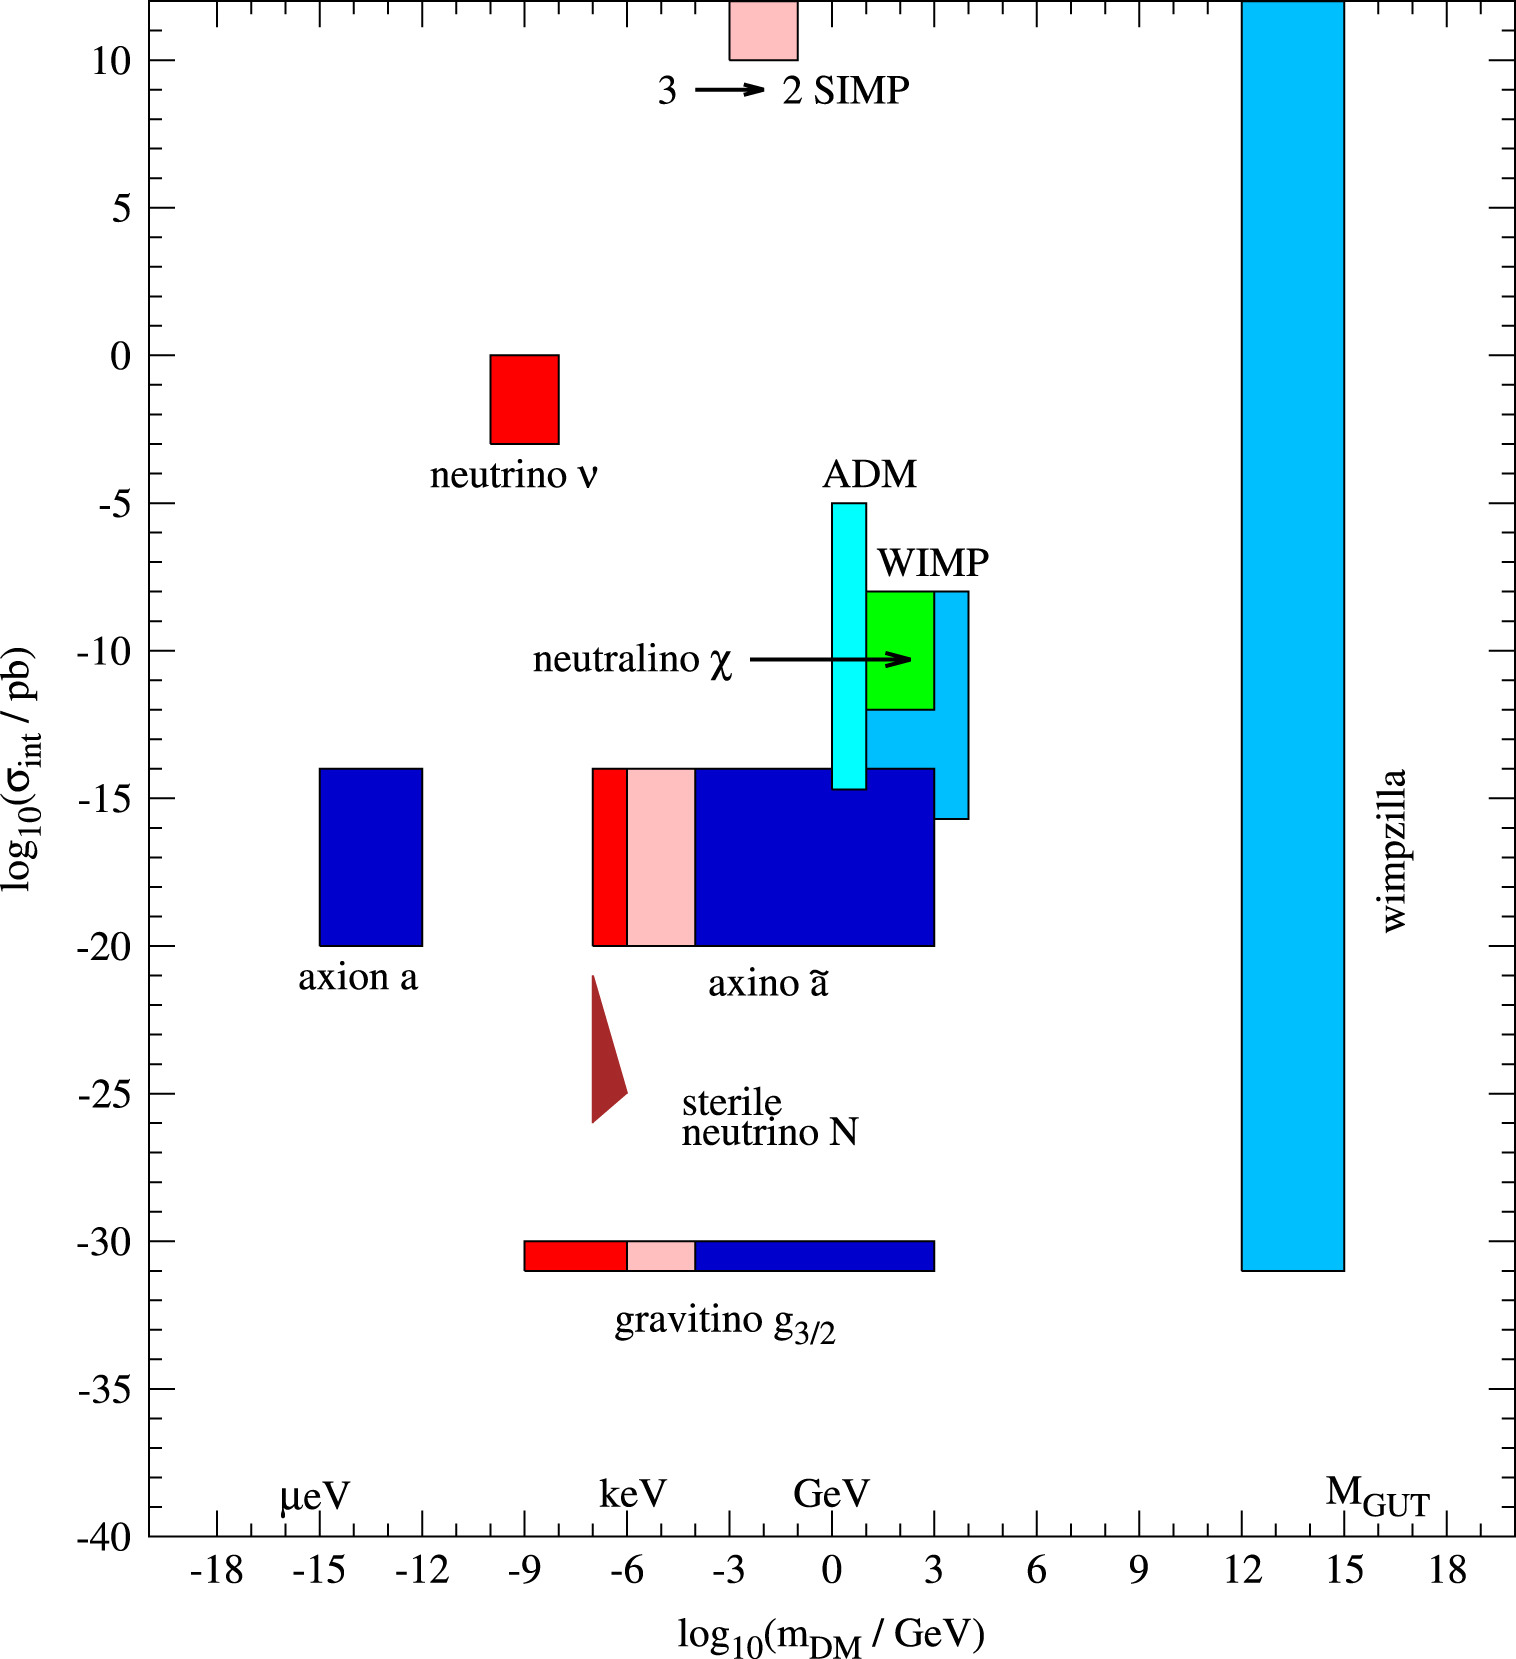
\includegraphics[scale=1]{images/mass_ranges.jpg}
\caption{\cite{BAER20151} Currently hypothesised masses for dark matter candidates from different theories.}
\label{fig:mass_ranges}
\end{figure}
\par Cosmological findings have been the driving motivation behind the dark matter search for the past 90 years \cite{bertone2018history}.
The leap to a Weakly Interacting Massive Particle (WIMP) \cite{steigman1984cosmological} is not a trivial one and one must take great care in the assumptions \cite{scherrer1986relic}
it makes and why they are made, especially in light of increasing ranges of masses being excluded by experiments running today.
The first defining feature is thus mass.
This is currently under heavy scrutiny of the scientific community as there are supporters of a very low mass dark matter candidate (such as axions \cite{weinberg1978new} or sterile neutrinos \cite{kusenko2009sterile})
while on the other side of the spectrum most standard direct detection experiments today \cite{Agnes_2015} \cite{McKinsey_2016}  are for mass ranges running from tens to hundreds of GeV/$c^2$.
Evidence from phenomena such as gravitational lensing \cite{wittman2000detection} and the constant rotational velocities of stars in galaxies with increasing
distance to their galactic centres \cite{oort1932force} suggest a candidate of dark matter halos around these celestial objects.
\\
\par From supersymmetrical neutralinos to superheavy dark matter candidates we are looking at a range from GeV/$c^2$ to
 several TeV/$c^2$, and even higher in certain theories \cite{roszkowski2004particle}, see Figure \ref{fig:mass_ranges}.
However, many of these theories share the production of WIMP candidates as a byproduct or as required assumptions
to allow their theories to work.
This strengthens the theory that such a particle should exist and what regions of mass, energy and interaction type to look for.
WIMPs are hypothesised to have been in thermal equilibrium with thermal plasma in the early universe.
As the universe expanded and WIMP annihilation rate was less than the Hubble expansion rate, the relic density for dark matter was reached.
Cross-sections expected for such WIMPs vary from theory to theory, however, are expected to be in the order of the weak interaction.
\\
\par The very low interaction rates with baryonic matter make it a challenge to detect such WIMPs.
There have been efforts at the Large Hadron Collider \cite{aad2013search} \cite{chatrchyan2012search}
to detect such elusive particles.
Single jet events were analysed with missing energies and transverse momenta which could only be
explained through a missing new particle in the mass range of a dark matter candidate.
Although, to date, these efforts have only translated into constraints of cross sections and mass, the search is still active.
\\
\par Another method of search is through indirect detection \cite{gaskins2016review} by observing celestial objects having a high mass to luminosity disparity.
Such objects include, but are not limited to, galactic centres, dwarf galaxies and galaxy clusters close to ours \cite{harvey2015nongravitational}.
Indirect detection relies on closely monitoring the particle flux coming from these objects verifying if self-interactions or decays into measurable standard model particles have occurred.
Searches via these methods are made even harder by the fact that the only byproducts most experiments can reliably measure (after accounting
for interstellar magnetic fields, other celestial objects and low background limits) are neutrinos and specific gamma ray energies.
\\
\begin{figure}[H]
\centering
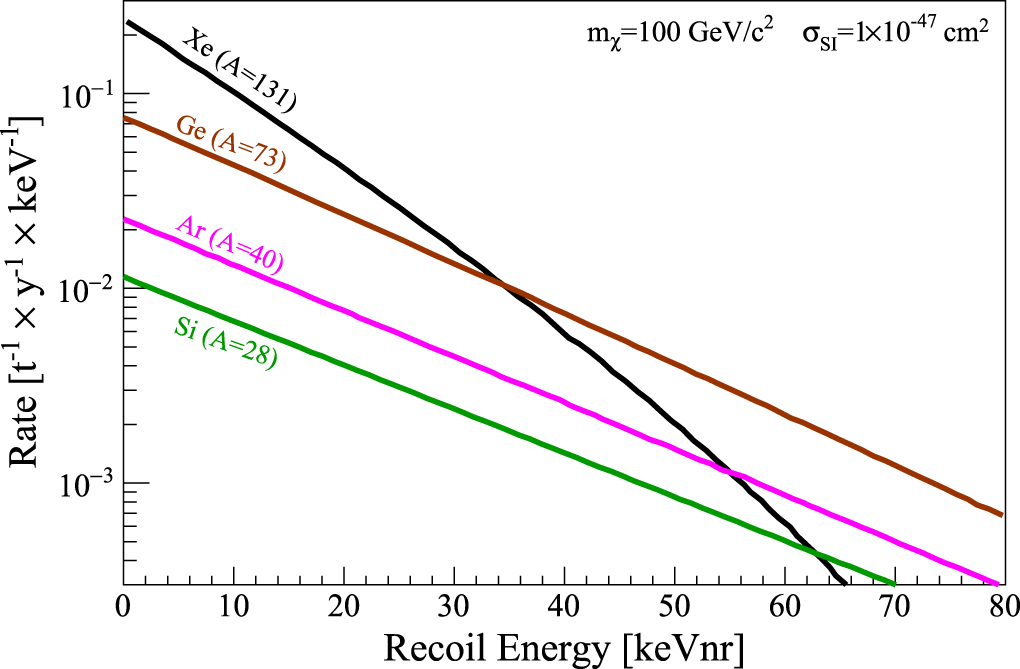
\includegraphics[scale=1]{images/recoil_spectra.jpg}
\caption{\cite{Schumann_2019} Nuclear recoil spectra for varying noble gas targets highlight the better interaction
rate at lower nuclear recoil energies for heavier targets but a lower rate for higher recoil energies.}
\label{fig:recoil_spectra}
\end{figure}
\par The last method of detection and the most common one as of today's experiments is direct detection \cite{gaitskell2004direct}.
Large detector chambers are set up, often many kilometers under the earth, essentially waiting for a WIMP
candidate to recoil elastically with a noble element atom and produce measurable scintillation.
For a WIMP mass ranging between 1 GeV/$c^2$ and 1000 GeV/$c^2$ recoil energies are in the range 1-100 keV
after which cross-sections become way too low for modern detectors.
The choice of noble gas element is also non-trivial, since, the rate for spin-indipendent interactions increases with
nucleon number, however, decreases at high energies due to form factor suppression, as expressed by \cite{goodman1985detectability}
\begin{equation}
\frac{{\rm{d}}{R}}{{{\rm{d}}{E}}_{\mathrm{nr}}} = \frac{\rho_0}{m_{\chi} m_N} \int_{v_{min}}^{v_{esc}}\frac{{\rm{d}}{\sigma_{x N}}}{{{\rm{d}}{E}}_{\mathrm{nr}}}(v,E_{\mathrm{nr}}) v f(v) dv,
\label{eq:dm}
\end{equation}
often approximated to \cite{lewin1996review}
\begin{equation}
\frac{{\rm{d}}{R}}{{{\rm{d}}{E}}_{\mathrm{nr}}}\propto \exp (- \frac{{E}_{\mathrm{nr}}}{{E}_{0}} \frac{4{m}_{\chi }{m}_{N}}{{({m}_{\chi }+{m}_{N})}^{2}})
\end{equation}
and shown in Figure \ref{fig:recoil_spectra} for increasing mass of the target nucleus.
Here $m_{\chi}$ is the dark matter mass, $m_N$ is the mass of the noble element, $\rho_0$ is density of dark matter in our local space,
$v_{min}$ is the dark matter velocity and depends on the annual and diurnal modulation \cite{drukier1986detecting}.
\\
\par The higher interaction rate for lower recoil energies makes it more probable to detect a WIMP candidate interaction, although these energies produce a lower intensity of scintillation.
Such low scintillation results in larger errors
(from sources such as photomultiplier calibration, photon efficiency, dark currents), so a compromise must be made.
Therefore, nuclear recoil energies are directly related to our algorithms since they directly affect the dark matter regime under study.
With the use of Monte Carlo simulators such as G4DS (Geant 4 DarkSide), one has to incorporate the nuclear recoil spectrum in the simulation setup
from which the program samples the $^{40}\mathrm{\text{Ar}}$ recoils.
This process is a long one since this program simulates everything from the interaction to detection and
can take several days if running over many energies with all the scintillation being captured.
\\
%\par Similarly, our machine learning algorithm is trained uniformly across the different energies but the choice of
%dark matter regime to be studied can be changed after training directly through the interaction rate distribution by choosing a suitable nuclear recoil spectrum.
%This is where the real advantage presented by this deep learning approach comes into play since the training is done once and changing
%sampling distribution can be done virtually instantly and does not require retraining.
%\\
\begin{figure}[H]
\centering
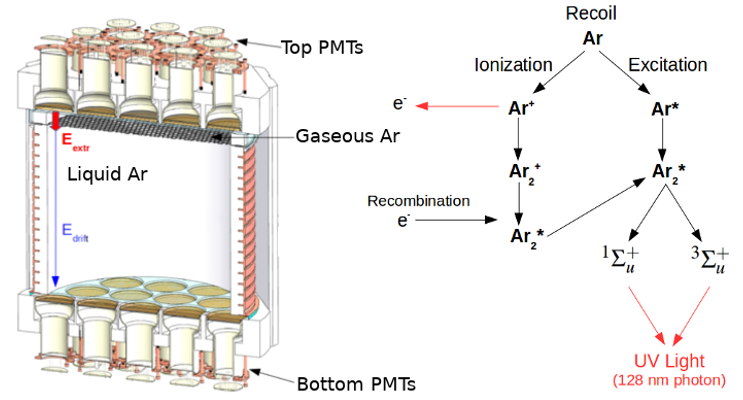
\includegraphics[scale=0.5]{images/detector.png}
\caption{\cite{edkins2017detailed} Schematic of a LAr-TPC and processes of VUV photon emission.}
\label{fig:detector}
\end{figure}
\par To understand the variables of interest in this study consider Figure \ref{fig:detector}.
A dark matter particle enters the detector fiducial volume where it interacts via the weak force with an $^{40}\mathrm{\text{Ar}}$ nucleus.
The latter becomes excited and during de-excitation emits electrons and produces scintillation denote by $S_1$ and having a window of observation of 7$\mu$s.
The electrons released drift upwards, due to an electric field, and take around 376$\mu$s to reach the top of the liquid Argon.
There, they reach a boundary between Argon in the liquid and gaseous phase which produces a secondary (much more intense) scintillation.
Subsequently, these photo-electrons are detected by Silicon photomultiplier tubes (SiPMTs) and are known as $S_2$;
the window of observation here is about 30$\mu$s.
The ratio of ionization to scintillation is lower for nuclear recoils
 than for electron recoils and, therefore, can be used to place selection cuts to increase sensitivity of the detector.
\\
\par There is a further variable used in the discrimination between background (electron recoils) and nuclear recoils.
Known as pulse shape discrimination, it relates to the de-excitation modes of the Argon nucleus post-recoil.
As illustrated by Figure \ref{fig:detector}, there are two excited states $^{1}\mathrm{{\Sigma_{u}}^{+}}$ and $^{3}\mathrm{{\Sigma_{u}}^{+}}$.
The former has a lifetime of 7ns, while the latter has a lifetime of 1600ns.
This difference makes Argon a very competitive candidate as a noble element target since, this same difference in lifetimes between
excited states in Xenon (the other major competitor for choice of noble element), is only of about 25ns.
Although Xenon has other benefits and Argon has other sources of background Xenon based dual phase TPCs do not have, for LAr-TPC based
detectors this feature is a very good discriminant.
This is due to the fact that the ratio of these excited state lifetimes is related to the stopping power or deposited energy per unit path length
$\frac{dE}{dx}$.
Such stopping power differs between electron recoils (from gamma photons or alpha particles) and
nuclear recoils (with Argon ion tracks).
Thus, a parameter called the Pulse Shape Discriminant is used and denoted by $f$ subscripted by the window of time of interest in ns.
We shall use $f_{200}$ defined as
\begin{equation}
f_{200}=\frac{\int_{0}^{200ns}\text{Intensity of photons received}}{\int_{0}^{7\mu s}\text{Intensity of photons received}}.
\end{equation}
Illustrated in Figure \ref{fig:psd} is the simulated difference in DarkSide-20k between nuclear and electron recoils for $f_{200}$ against total $S_1$ intensity.
Although historically the parameter $f_{90}$ has been used for experiments such as DarkSide-50, for a much bigger experiment such as this, the drift distance is increased substantially so
$f_{200}$ is more suitable.
\begin{figure}[H]
\begin{minipage}{.49\textwidth}
  \centering
  \begin{subfigure}{\textwidth}
      \centering\captionsetup{width=.9\linewidth}%
      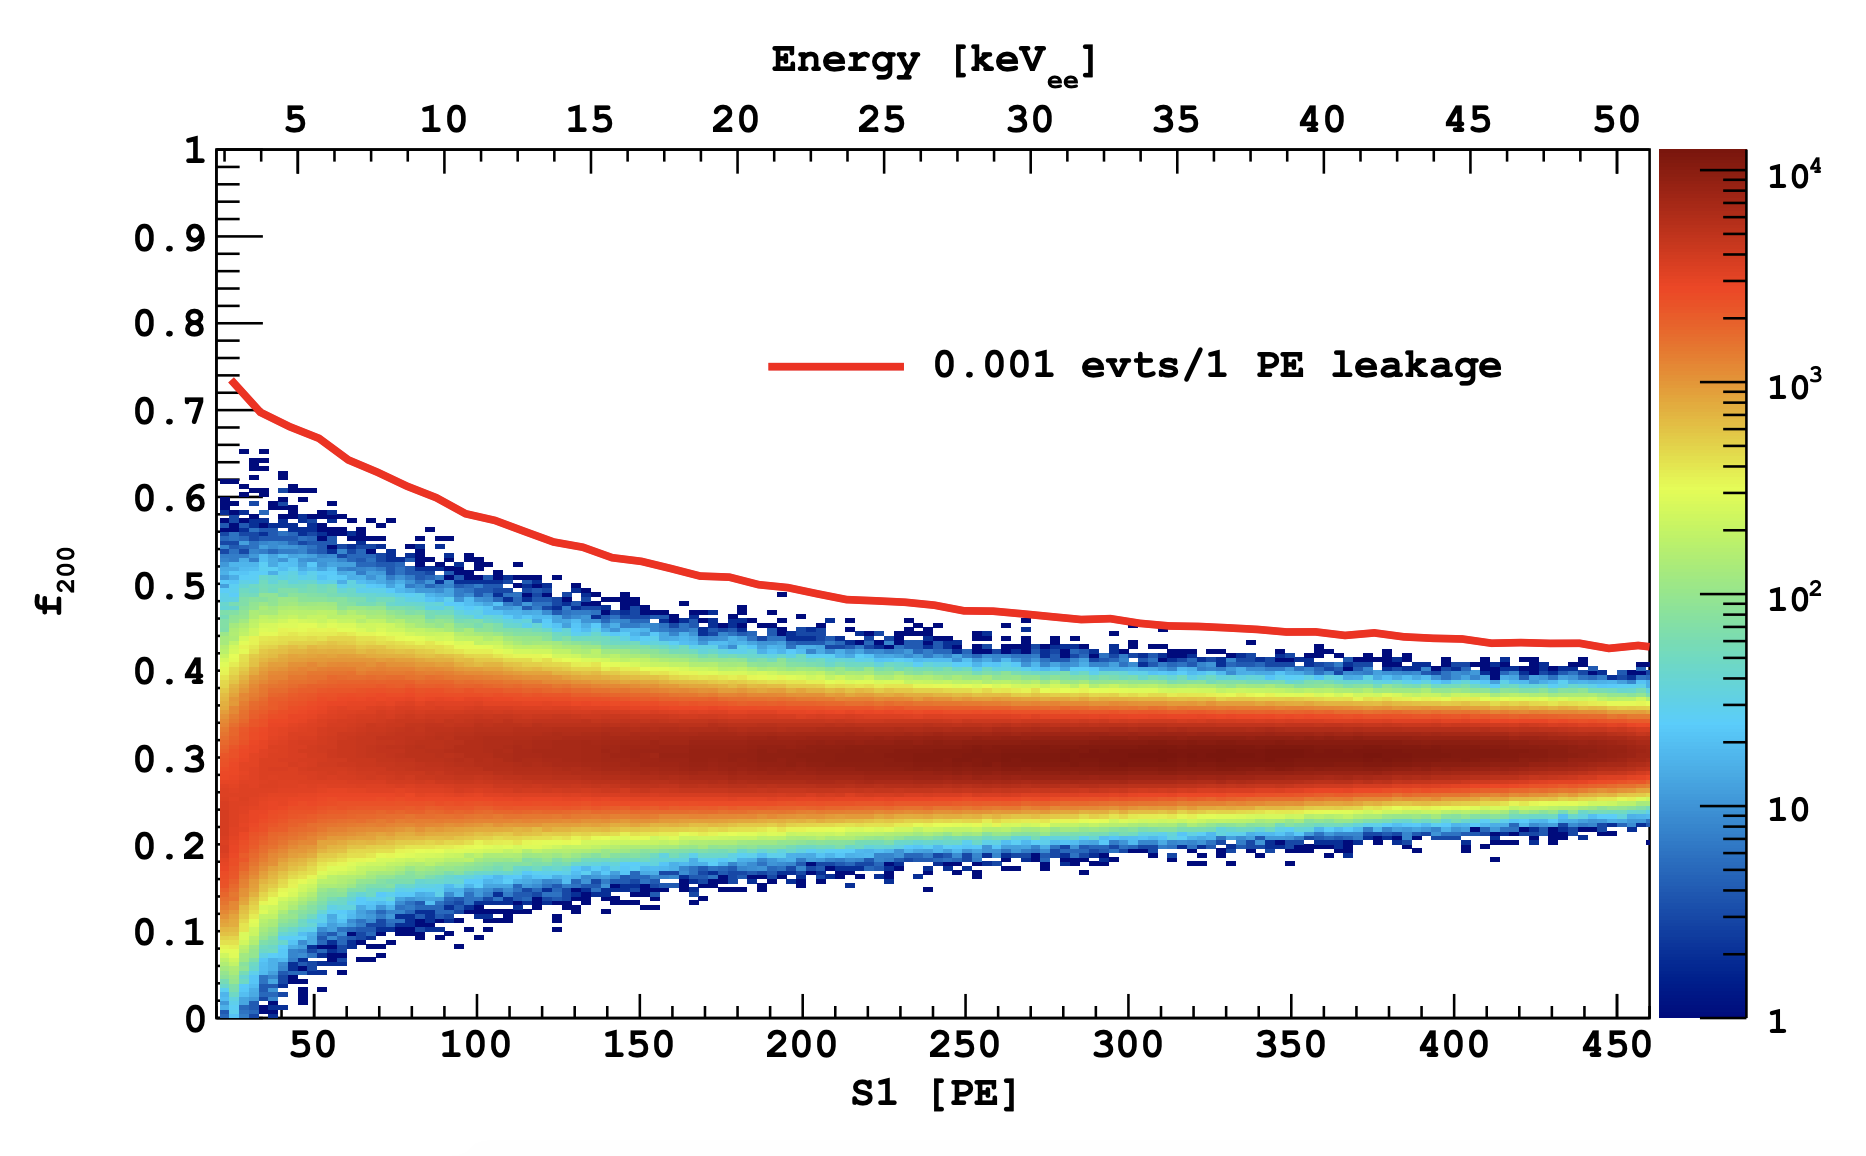
\includegraphics[width=\textwidth]{./images/psd_background.png}
      \caption{Simulations for DarkSide-20k of $f_{200}$ vs $S_1$ for background data using $^{39}\mathrm{\text{Ar}}$ $\beta$'s.
      Red line is a leakage curve for a 5-PE requirement on $\beta$'s.}
  \end{subfigure}
\end{minipage}
\begin{minipage}{.49\textwidth}
  \centering
  \begin{subfigure}{\textwidth}
      \centering\captionsetup{width=.9\linewidth}%
      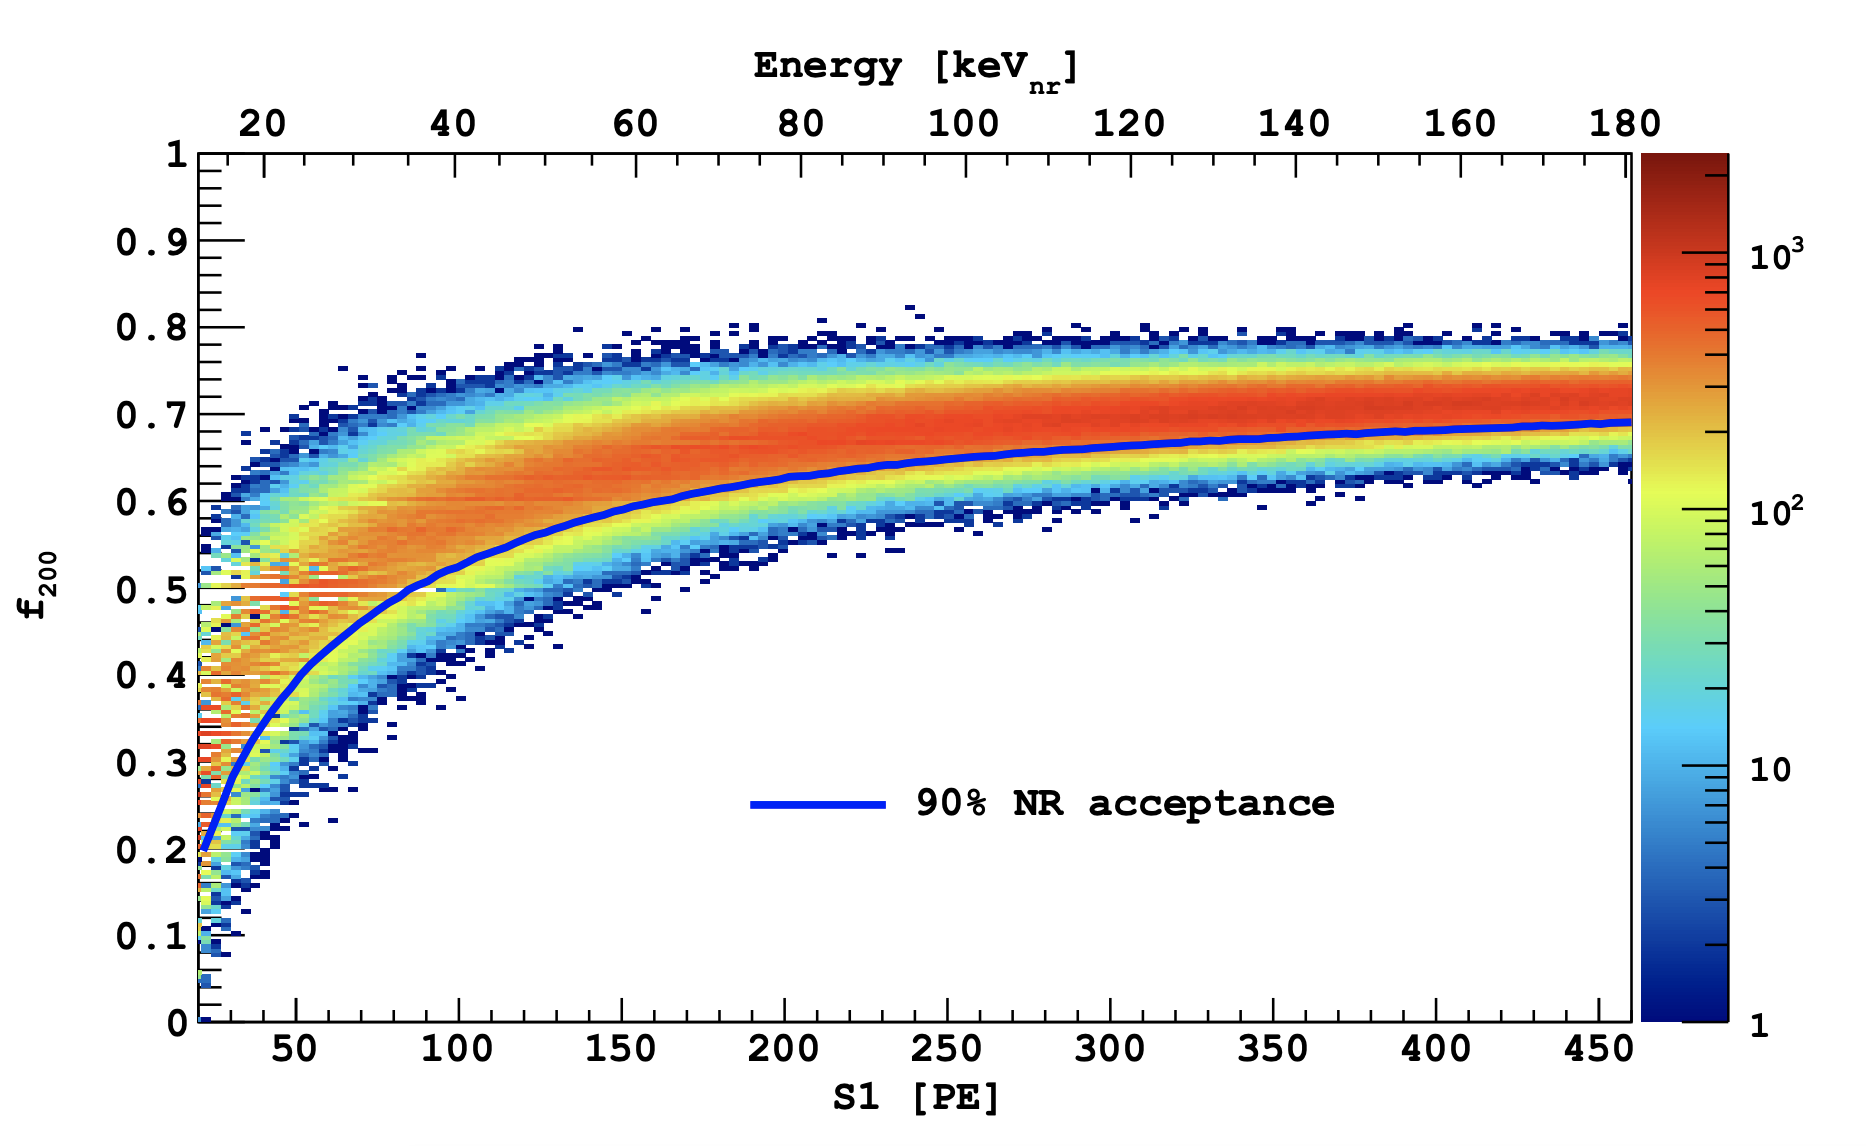
\includegraphics[width=\textwidth]{./images/psd_signal.png}
      \caption{Simulations for DarkSide-20k of $f_{200}$ vs $S_1$ for signal nuclear recoils.
      Blue curve is the 90\% NR acceptance region.}
  \end{subfigure}
\end{minipage}
\caption{\cite{aalseth2018darkside} Region of interest using $f_{200}$ pulse shape discriminant against total intensity $S_1$.}
\label{fig:psd}
\end{figure}
\subsection{Current G4DS Results}
The current simulation methods used by the DarkSide collaboration consist of very sophisticated and proven Monte Carlo methods.
They have been programmed using an open-source software package called Geant4 \cite{G4} and the complete set of detector macros and routines is called G4DS.
For the purposes of this report and our algorithms, we ran G4DS with the following configuration detailed in Table \ref{table:g4ds_config}.
\begin{table}[!th]
\centering
\begin{tabular}{l|l}
\hline
Drift Field & 200V \\
TPC Height & 262cm \\
TPC Width & 150cm \\
Thickness Acrylic Walls & 5cm \\
Thickness LArBuffers & 40cm \\
Thickness Veto Shell & 10cm \\
Thickness TPB & 0.1 mm \\
\hline
\end{tabular}
\caption{Table detailing the major features of the detector setup used in G4DS for the purposes of this study.}
\label{table:g4ds_config}
\end{table}
\\
\par Although the default configuration was used, no selection cuts were made on any of the data for the purpose of simply studying the reproducing power of the deep learning technique.
We simulated 1000 uniformly distributed $^{40}\mathrm{\text{Ar}}$ recoils for each energy in the range [5,235] keV in steps of 1 keV.
An example for 1000, 100 keV nuclear recoil events is shown in Figure \ref{fig:example_vars} for each of the three variables $S_1$, $S_2$ and $f_{200}$.
The data for each variable is similar in shape, but the ranges are different and the separation in means for the 200 different energies is quite small for $f_{200}$
when compared to $S_1$ and $S_2$.
Thus, there might be difficulty in training a neural network to produce such $f_{200}$ distributions
 solely on condition of the energy, since they are not very distinguishable from each other and do overlap.
The neural networks described in the next section were trained on these types of distributions and the final aim was to reproduce
plots such as Figure \ref{fig:psd}, to verify whether the correlation between the three variables was understood.

\begin{figure}[H]
\begin{minipage}{.5\textwidth}
  \centering
  \begin{subfigure}{.9\textwidth}
      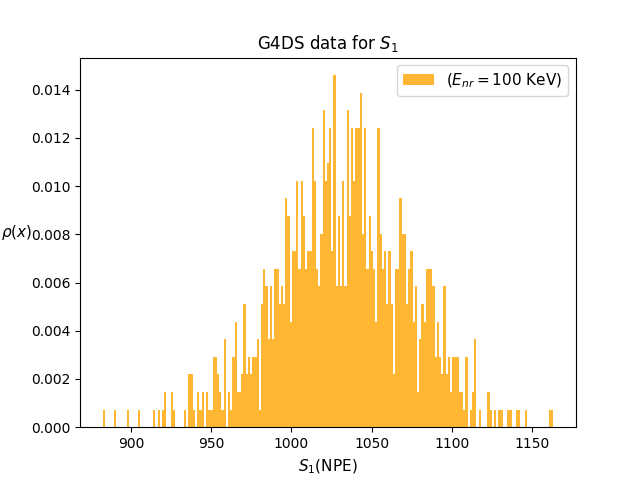
\includegraphics[width=\textwidth]{./images/s1_100.png}
      \subcaption{G4DS generated data for $S_1$}
  \end{subfigure}
\end{minipage}
\begin{minipage}{.5\textwidth}
  \centering
  \begin{subfigure}{.9\textwidth}
      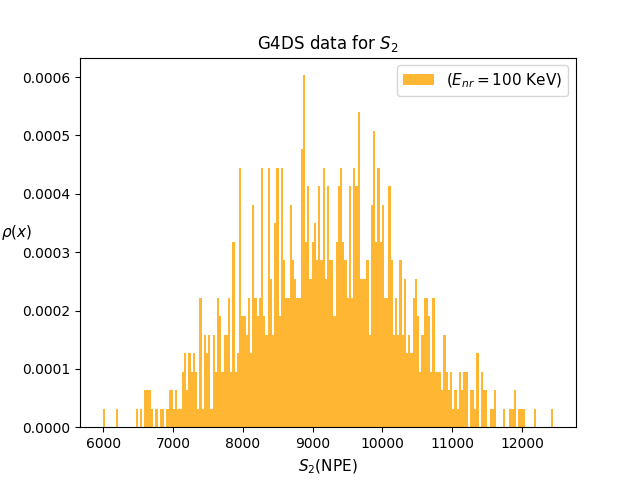
\includegraphics[width=\textwidth]{./images/s2_100.png}
      \subcaption{G4DS generated data for $S_2$}
  \end{subfigure}
\end{minipage}
\end{figure}
\begin{figure}[H]\ContinuedFloat
\centering
\begin{minipage}{.5\textwidth}
  \centering
  \begin{subfigure}{.9\textwidth}
      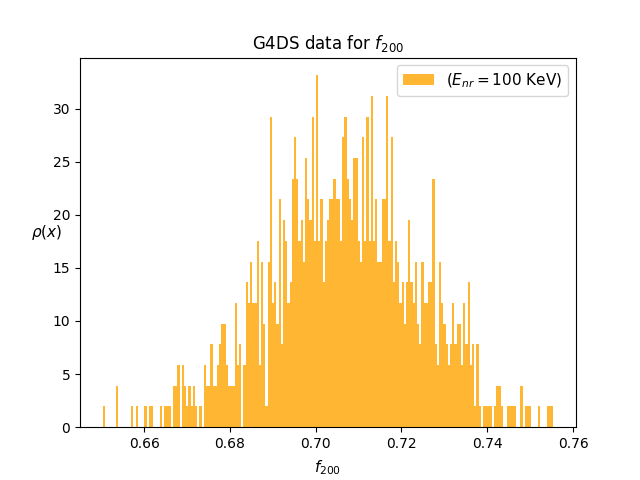
\includegraphics[width=\textwidth]{./images/f200like_100.png}
      \subcaption{G4DS generated data for $f_{200}$}
  \end{subfigure}
\end{minipage}
\caption{Example of the generated data for a run of 1000, 100 keV $^{40}\mathrm{\text{Ar}}$ elastic nuclear recoils in G4DS.}
\label{fig:example_vars}
\end{figure}

\subsection{Deep learning as an alternative}
As discussed earlier, the results obtained from G4DS are well understood and accepted as the \textit{de facto} simulations (backed up by experiments DS50 \cite{agnes2015first}).
However, with great detail come large amounts of time waiting for the simulations to complete.
Moreover, anytime the nuclear recoil spectrum is changed to simulate different masses of WIMPs, the simulations must be re-run. This
 hinders the rate at which research progress can be made, since, instead of being able to test multiple theories,
  one must take great care to compromise with the time spent waiting and computational resources needed.
A solution could possibly be to increase the number of processors, GPUs and computing capabilities, however,
 these come at a cost and do not necessarily scale linearly.
\\
\par This is where neural networks appear as a possible, scalable solution to the problem.
The following is a quick overview of some of the most important machine learning concepts, useful in understanding our work.
For a more complete introduction to machine learning techniques please refer to my first semester report \cite{firstsemester}.
A neural network is a set of nodes (vectors of numbers) in different, successively connected layers.
Each layer contains many nodes connected via mappings to other nodes from successive and previous layers.
Each of these nodes carry intermediary weights to certain functions of output.
In a single forward run (known as an epoch), the input layers (containing the data to be trained) are connected to
intermediary layers.
In turn, these carry out some transformation applying a so called 'activation function' to give
the intermediary weights some values.
The process is repeated until the final layer is reached.
The latter will usually have an activation function dependent on the type of problem at hand.
For example, a classification problem will have weights representing each category.
The largest value will be for the category the algorithm classifies the input as, and lower or 0 for the others.
The final weights are then compared to what they should be (from the known labelled training data)
 and a quantity to measure 'goodness' of the algorithm, called the loss, is calculated.
The function doing this measure is called the loss function.
An optimizer acts on the value of the loss and changes the intermediary weights accordingly.
The aim is that on the next run/epoch
the new weights and activation functions will guide the algorithm towards better
final weights, in order to minimize loss and maximise accuracy.
\\
\par The aforementioned is a type of machine learning known as supervised learning.
The other kind, unsupervised learning, is what we carry out in the algorithms detailed in this report,
 where, we essentially implement dimensionality reduction.
Dimensionality reduction is the transformation from data space,
 which has often has many dimensions, to a meaningful representation easier to manipulate.
Particularly, we make use of a rather new method of machine learning known as Generative Adverserial Networks \cite{NIPS2014_5423} \cite{salimans2016improved}.
In our case we have two neural networks: one known as the classifier and the other as the generator.
The aim of the generator is to reproduce training data as closely as possible whilst the job of the classifier is to
spot, at each epoch, which of the two inputs it is being presented with; real or generated.
Their loss functions, for a fixed generator G and the optimal discriminator $D^*_G(\bar x)$ is given by minimizing the function \cite{NIPS2014_5423}
\begin{equation}
  C(G)=\E_{x\sim p_{data}}[\log (D^*_G(\bar x)]+\E_{x\sim p_{g}}[\log(1-D^*_G(\bar x)]
  \label{eq:minmax}
\end{equation}
where the optimal discriminator is described by
\begin{equation}
  D^*_G(\bar x)= \frac{p_{data}(\bar x)}{p_{data}(\bar x) + p_{g}(\bar x)}.
  \label{eq:optimal_disc}
\end{equation}
\\
For the ideal case where the generator is perfect, the accuracy of the discriminator is expected to be
at around 0.5.
Here, it would have no better way, other than a 50\%-50\% chance, to tell the difference between real and generated data.
\section{Methods}
\subsection{Problems with previous approach}
In the first semester, a qualitative approach was taken in reproducing G4DS data through a GAN.
Moreover, we required a cGAN, or conditional GAN, which would accept as a condition the nuclear recoil energy E and produce the corresponding $S_1$, $S_2$, $f_{200}$.
The results of that report showed promising reproductions of the real data but this approach presented with three main problems:
\begin{enumerate}[i)]
  \item There was barely any quantitative analysis of the comparison between training data and the GAN output.
  This was done mainly by visually looking at any two same energy plots for a particular variable, since, the main aim was to verify whether such an algorithm could even be compiled.
  \item As we trained the GAN to learn $P(S_1|E)$, $P(S_1 \cap S_2|E)$ and so on, the network created was exponentially larger and more complicated.
  It was not only a matter of adding more layers or nodes but required a substantial rethinking of the networks (generator and discriminator) for each variable.
  \item The 3D, 1 conditional GAN (learning the 3 variables at once given 1 condition) was not successful and we quickly had to abandon this path since it did not produce any returns on effort put in.
\end{enumerate}
\subsection{Novel techniques}
\subsubsection{Wasserstein GANs}
As a result, we expanded our search for a different architecture of GANs.
At the end of last semester we identified wGANs, or Wasserstein GANs \cite{arjovsky2017wasserstein}, to be the next architecture we would try.
The main feature of this GAN is its use of a different loss function; the way of quantifying how bad the generator output is from the real data.
Contrary to our original belief (the difference being only about modifying the loss function and some minor tweaks in the code),
initial results quickly highlighted that we were dealing with a fundamentally different architecture.
This would have meant spending close to the same amount of time as the first
 semester only to get to the same point we had already.
This architecture promised better convergence in less epochs and is proven to be
much better in terms of performance than the minmax approach taken by the
underlying loss function of the traditional GAN.
However, this was not in line with the aim for this semester.
We thus decided to focus our efforts on other architectures.
Importantly, we are not implying wGANs are not worth implementing.
Rather, from what we observed during
proof of concept training, they are very efficient but easily end up in failure modes (described later) if not configured well.
So, we do suggest this architecture be studied in the future, perhaps in the next iteration of this project, since it could potentially
save many epochs worth of work and achieve even better convergence.
\subsubsection{ARGANs}
AutoRegressive GANs \cite{yazici2018autoregressive} \cite{zhao2019compression} have first been called so in 2018 although the underlying theory has been used in the context of machine learning for decades now.
Although mostly used in the ambit of image generation, the method still applies to our problem.
In reality, the ARGAN proposed in 2018 modelled data in the latent (feature) space rather than data space like the older
employers of this method did \cite{fu2019time}.
The closest to what we have done was performed in 2011 \cite{oord2016pixel} when a GAN was used by training it in an image generation context.
Each pixel was trained individually given as a condition all its preceding pixels.
Similarly the probability we are trying to teach our generator in this method is given by
\begin{equation}
  p(\bar x)= \prod_{i=1}^np(x_i|x_0,...,x_{i-1})
  \label{eq:prob_dist}
\end{equation}
where in our case $i$ runs from 1 to 3 for $S_1$, $S_2$, $f_{200}$ and $i=0$ is the recoil energy E.
More explicitly, $P(S_1|E)$ was taught for a number of epochs (usually 10,000 in this report) and the best output of that generator was
passed to $P(S_2|S_1,E)$ to be trained for a further 10,000 epochs and again to obtain $P(f_{200}|S_2,S_1,E)$.
Its massive advantage is that essentially we are training 1DcGANs (where the dimension is the number of variables being taught) and
by the end of the process we have trained the three variables with their joint probabilities, all from a single energy input.
Moreover, the complexity of this architecture is comparable to the 1D original cGAN rather than the 3D cGAN.
Lastly (in my personal opinion as an advocate for scalability and future-proofing) we are ensuring that if the collaboration's needs
are ever changed so as to require the need to train a further variable, this can be easily done.
Unless the new variable is wildly different than the three already taught, chances are, that a very similar neural network can be used.
\subsubsection{Moments as a measure of performance}
One of the conclusions from last semester was the need for more detailed metrics to compare generator and discriminator
performance while training.
We used to monitor performance using the discriminator accuracy/loss vs epoch curve.
Ideally, the accuracy would converge to about 0.5 and loss to about 0.7; beyond checking this convergence, those plots do not convey much information.
In fact, GANs suffer from failure modes whereby the accuracy/loss plot shows convergence but
the generated data is nowhere close the real data.
Mathematically, the generator and discriminator reach a Nash equilibrium \cite{salimans2016improved}
and thus the generator converges on wrong points in data space.
\begin{figure}[H]
\centering
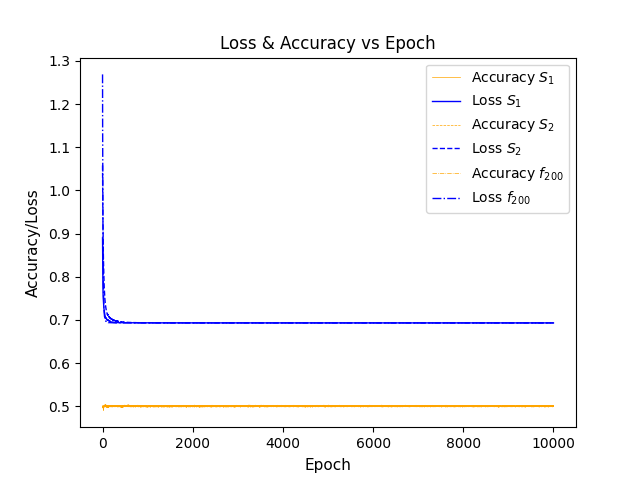
\includegraphics[width=0.65\textwidth]{./images/performance.png}
\caption{Previously used in semester 1, accuracy/loss curves clearly do not convey enough
information about convergence and performance of the GAN during training.
This particular run did not converge for $f_{200}$.}
\label{fig:acc_loss}
\end{figure}
\par
A new metric would not only allow us to better compare how different GAN configuration affect performance but also
give us the opportunity in real-time to gauge whether the current configuration in use is likely to converge.
We were in search of a fast method of metric elaboration so as not to hinder the already cumbersome process of training.
Although metrics such as Wasserstein distance are ideal, we carry them out after training in the analysis stage.
We also did not require granular detail about performance but needed a measure of how the GAN was performing, per variable, across the whole energy domain.
\\
\par Thus, we settled on selecting three energies from the whole 230 energy samples being simultaneously trained on.
These three energies were specifically selected to be the first, middle and last in the domain.
Then, the array of length 3 arrays, of length 1000 data points each, is flattened into a single array and the first and second moments are resolved.
The ratio of $\frac{\E(\text{GAN4DS Output})}{\E(\text{G4DS Output})}$ and $\frac{\Var(\text{GAN4DS Output})}{\Var(\text{G4DS Output})}$ is obtained.
Figure \ref{fig:moments} shows these ratios plotted at every epoch check (which in this run was at every 100 epochs) for the same run
as in Figure \ref{fig:acc_loss}, which ended up not converging for $f_{200}$.
It is fair to assert that Figure \ref{fig:moments} does a much better job at showing the non convergence than Figure \ref{fig:acc_loss}.
Our suggestion is these plots be used alongside the accuracy/loss curves since a convergence in the latter
but non convergence in the former is the best way to observe failure modes.
This is an added advantage of having these new plots.
\\
\par Finally, at every epoch check after logging these ratios, we also verify whether the current generator is the best one yet.
The way we do this is to use the Taxicab metric on the three histgorams for the recoil energies mentioned earlier (lowest, middle and highest in the domain)
between GAN4DS and G4DS and sum the distances for all three energies.
We then check if this is less than the previous sum of distances and, if it is, we save the weights to the current model.
This allows us to save the generator that, using the metric aforementioned, most closely resembles the training dataset.
At the same time, the neural network is trying to minimize the value of the loss.
As a potential extension, and given the promising results the ratio plots have shown us, we
suggest using this metric in the future by including it directly into the neural network layout as a metric alongside loss minimization.
\begin{figure}[H]
\centering
\begin{minipage}{\textwidth}
  \begin{subfigure}{.5\textwidth}
      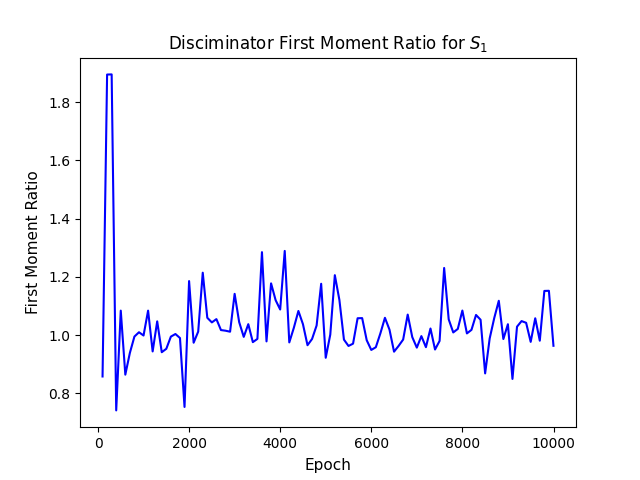
\includegraphics[scale=0.6]{./images/moment_1_s1.png}
      \subcaption{Ratio of first moment for $S_{1}$}
  \end{subfigure}
  \begin{subfigure}{.5\textwidth}
      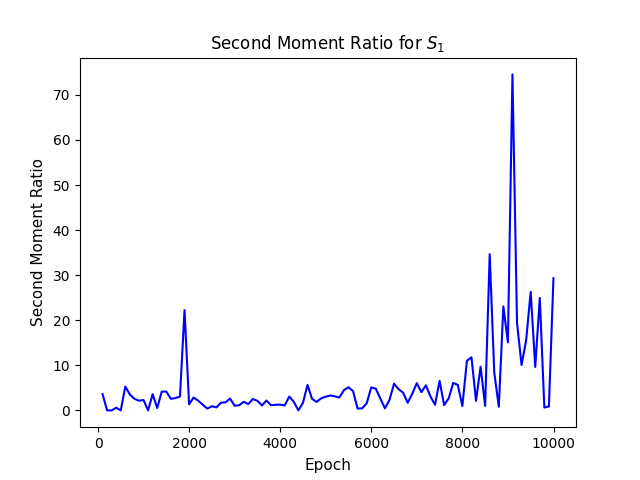
\includegraphics[scale=0.6]{./images/moment_2_s1.png}
      \subcaption{Ratio of second moment for $S_{1}$}
  \end{subfigure}
\end{minipage}
\begin{minipage}{\textwidth}
  \begin{subfigure}{.5\textwidth}
      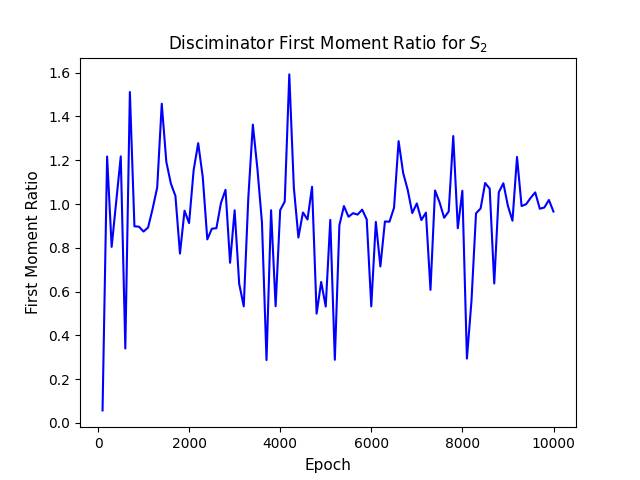
\includegraphics[scale=0.6]{./images/moment_1_s2.png}
      \subcaption{Ratio of first moment for $S_{2}$}
  \end{subfigure}
  \begin{subfigure}{.5\textwidth}
      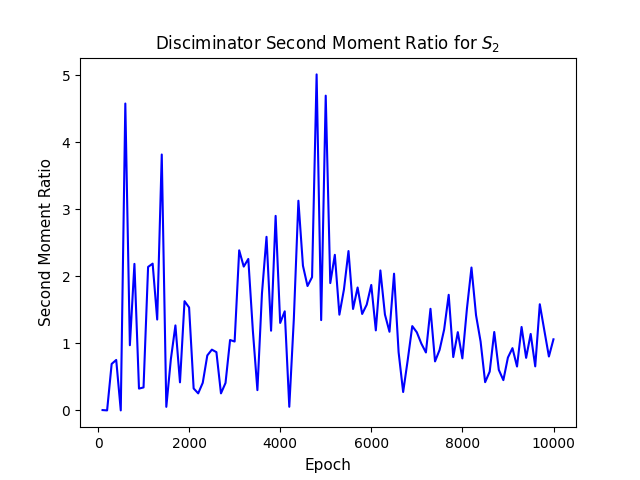
\includegraphics[scale=0.6]{./images/moment_2_s2.png}
      \subcaption{Ratio of second moment for $S_{2}$}
  \end{subfigure}
\end{minipage}
\begin{minipage}{\textwidth}
  \begin{subfigure}{.5\textwidth}
      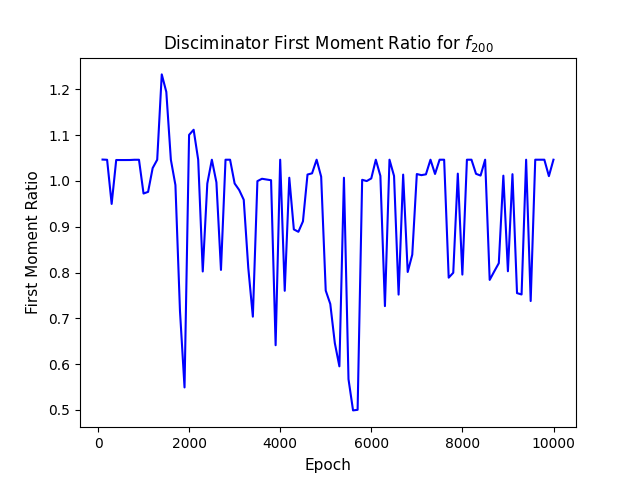
\includegraphics[scale=0.6]{./images/moment_1_f200like.png}
      \subcaption{Ratio of first moment for $f_{200}$}
  \end{subfigure}
  \begin{subfigure}{.5\textwidth}
      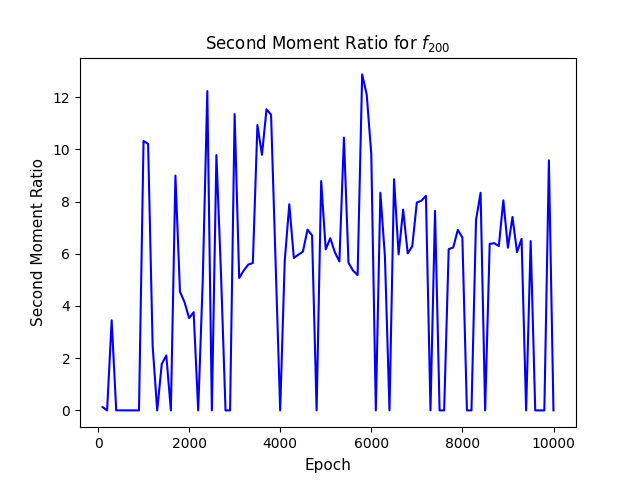
\includegraphics[scale=0.6]{./images/moment_2_f200like.png}
      \subcaption{Ratio of second moment for $f_{200}$}
  \end{subfigure}
\end{minipage}
\caption{Use of ratio of GAN4DS/G4DS moments for three test recoil energies during training drastically improves the capture of the actual performance of the GAN
compared to accuracy-loss more commonly used in machine learning.}
\label{fig:moments}
\end{figure}
\subsubsection{Work Pipeline}
Before presenting final results, I thought it might be worthwhile briefly mentioning how we obtained them via
changes to our coding styles and the way we completely redefined our work pipeline.
Last semester we worked on an online, free platform provided by Google called Colab.
This helped us work together by sharing the same results and make use of the Python Jupyter notebooks with NVIDIA T4 GPUs which have a 16GB memory;
a much needed resource for the large dataset of training we employ.
However, we easily found ourselves with tens of notebooks, each with a different architecture needing manual saving of the outputs.
Consistency between different notebooks was lacking at best and the biggest drawback was that the session would timeout after a while so the network could not
be let to train for long periods of time reliably.
\\
\par Therefore, we took the opportunity to convert all of the code to a single Python 3 project to be run on the University of Manchester's Physics Department GPU cluster.
The package we produced aims on being able to be easily used in the future by people that might not be aware of the inner workings of machine learning.
Instead, it shifts the focus on what the researcher needs to train on and the desired output.
The program takes in the variables, the training dataset (after self-extracting from ROOT files of $\approx$ 1GB per energy to $\approx$ 20kB)
and a layout specified in a markup language independent from the Python code.
Then, the program automatically splits up the data in as many batches as needed to serve memory requirements, creates the ARGAN structure, opens a monitorable
Tensorboard session and saves all plots and data logs in a single, consistent format.
Tensorboard is a package provided by Google which allows monitoring machine learning progress to the level
where one can see the weights of each individual layer to monitor how they change with epochs.
We actually made use of this to remove any layers or nodes which were essentially useless or redundant or,
 in certain cases, were damaging performance and convergence.
We made this codebase in the hope it could serve as a baseline for future teams,
 potentially working on continuing our work.
Thus, we encourage to expand its capabilities and change it as needed.
\section{Results}
All results, unless specified otherwise, were obtained using an ARGAN with 10,000 epochs per variable.
The dataset is comprised of 1000 $^{40}\mathrm{\text{Ar}}$ recoils per nuclear recoil energy in the range [5,235] keV in steps of 1 keV.
The order of variables learnt was $S_1$ then $S_2$ then $f_{200}$.
All results presented are from the same run with the above configuration.
\subsection{Individual Variables}
The first results I present are the individual variables.
Figure \ref{fig:ind_results} shows (left) the results of 3 nuclear recoil energies (minimum, middle and maximum over the recoil energy domain)
of training dataset overlayed with the best GAN output per variable and
(right) the differences for each two equal energy, equal variable counts.
Figure \ref{fig:ind_results_metrics} shows the metrics used to monitor performance during training.
\\
\par The difference plots seem to show a symmetry about the mean of each training dataset distribution.
The GAN appears to have produced output which on one side under-estimates the training data and over-estimates it
on the other side.
The largest difference is seen in the lower energies of the $f_{200}$ distribution.
This could be attributed to the much more spread-out shape these lower energies have when compared to the larger energies.
GANs are known to suffer in datasets where there is high variance across members \cite{yazici2018autoregressive}.
\begin{figure}[H]
\centering
\begin{minipage}{\textwidth}
  \begin{subfigure}{.5\textwidth}
      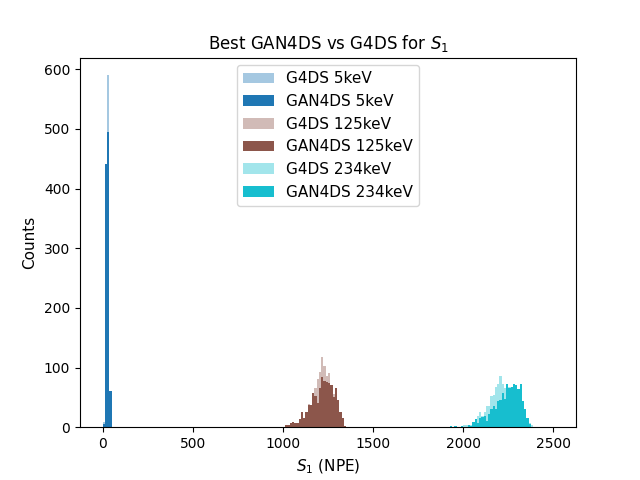
\includegraphics[scale=0.6]{./images/best_s1.png}
      \subcaption{GAN4DS overlayed with G4DS for $S_1$.}
  \end{subfigure}
  \begin{subfigure}{.5\textwidth}
      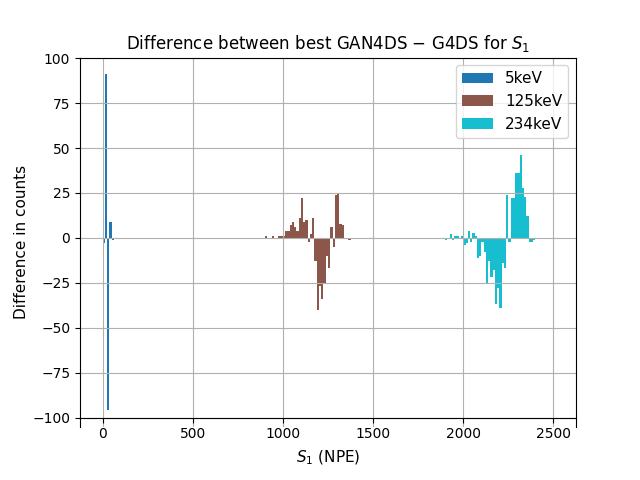
\includegraphics[scale=0.6]{./images/difference_best_s1.png}
      \subcaption{Difference plots for GAN4DS$-$G4DS for $S_1$.}
  \end{subfigure}
\end{minipage}
\begin{minipage}{\textwidth}
  \begin{subfigure}{.5\textwidth}
      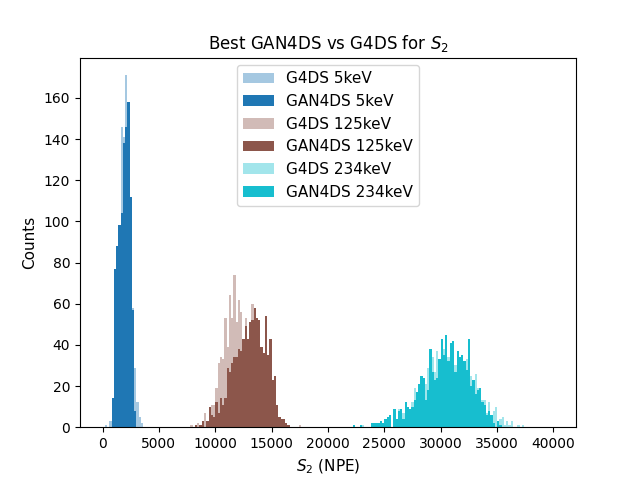
\includegraphics[scale=0.6]{./images/best_s2.png}
      \subcaption{GAN4DS overlayed with G4DS for $S_2$.}
  \end{subfigure}
  \begin{subfigure}{.5\textwidth}
      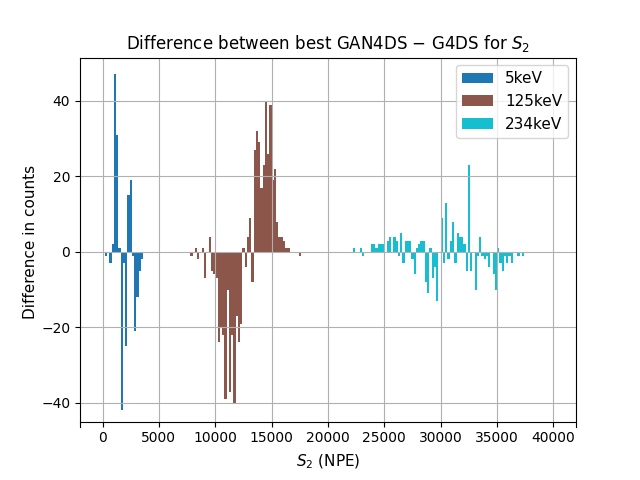
\includegraphics[scale=0.6]{./images/difference_best_s2.png}
      \subcaption{Difference plots for GAN4DS$-$G4DS for $S_2$.}
  \end{subfigure}
\end{minipage}
\begin{minipage}{\textwidth}
  \begin{subfigure}{.5\textwidth}
      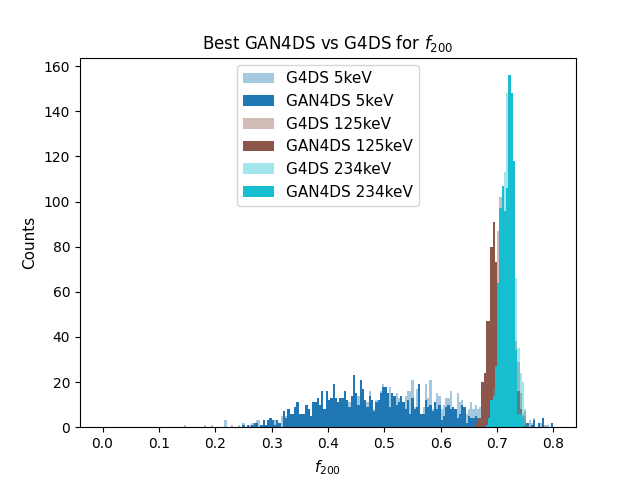
\includegraphics[scale=0.6]{./images/best_f200like.png}
      \subcaption{GAN4DS overlayed with G4DS for $f_{200}$.}
  \end{subfigure}
  \begin{subfigure}{.5\textwidth}
      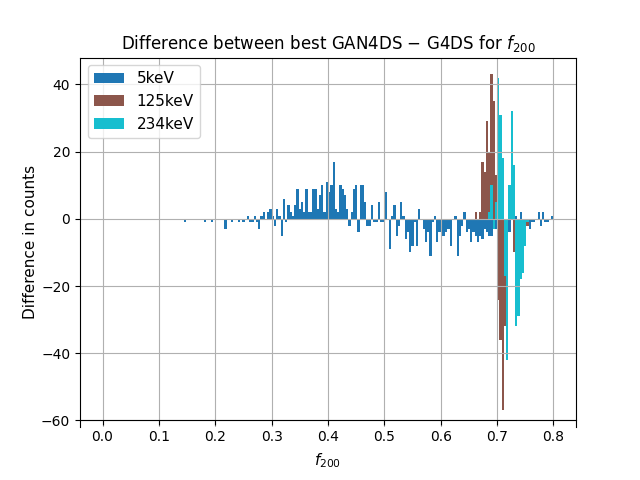
\includegraphics[scale=0.6]{./images/difference_best_f200like.png}
      \subcaption{Difference plots for GAN4DS$-$G4DS for $f_{200}$.}
  \end{subfigure}
\end{minipage}
\caption{Individual variables learnt successively with each variable adding itself as an input condition
to the next variable being trained. Direct comparisons between generated and trained data to the left, differences per bin on the right.}
\label{fig:ind_results}
\end{figure}
\newpage
\null
\vfill
\begin{figure}[H]
\centering
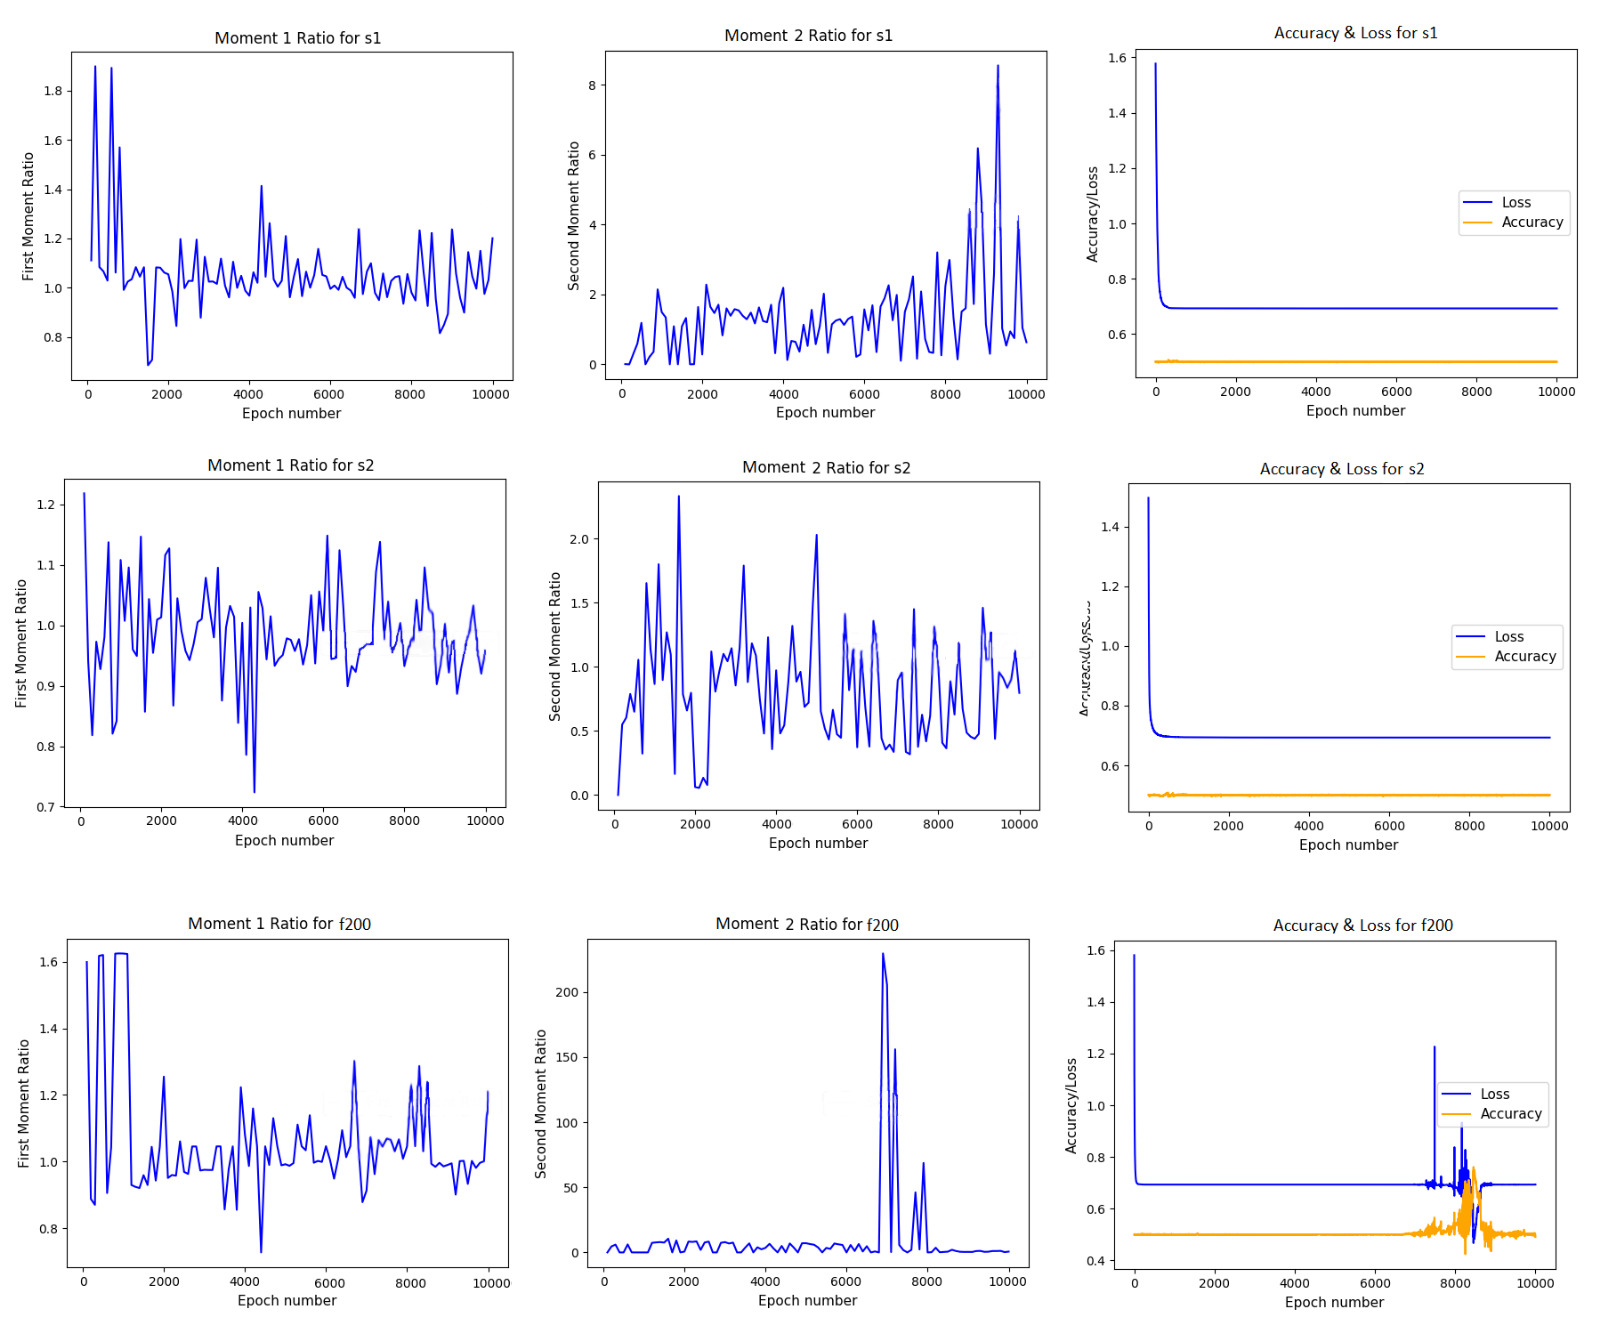
\includegraphics[scale=0.3]{./images/working_metrics.jpeg}
\caption{The metrics used during training to capture performance and convergence
of the GAN on training data.
 From the accuracy/loss plot and the moments plots it appears the GAN had entered a failure mode for $f_{200}$ but
 comes out of it to converge on the actual training data at around 8000 epochs.}
\label{fig:ind_results_metrics}
\end{figure}
\null
\vfill
\newpage
\subsection{Variable Correlations}
Although individual variables are very important, we mainly sought out to teach the GAN the correlations between them.
Figures \ref{fig:corr_results_1_5} (log$(m)=1.5$) and \ref{fig:corr_results_4} (log$(m)=4$) show the results for correlations between
the individual variables shown previously.
To produce these correlation plots first a mass for the WIMP is chosen, in this case we take log$(m)=1.5$ and log$(m)=4$ in a spin-independent model which corresponds to a 31.5 GeV/$c^2$ mass.
From theory the corresponding recoil energy spectrum is chosen, shown by Figure \ref{fig:recoil} for log$(m)=$1.5.
From this, 1000 recoil energies are sampled to select from the different runs , both in G4DS and GAN4DS.
\begin{figure}[H]
\centering
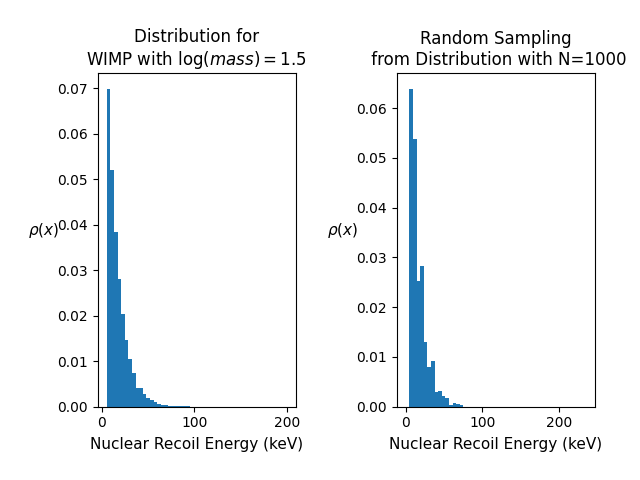
\includegraphics[scale=0.6]{images/Ar_c1dat_m1-5.png}
\caption{A plot of the theoretical recoil energy spectrum for a WIMP of mass log$(m)=1.5$ vs the
sampled N=1000 energies spectrum. The same is done for log$(m)=4$.}
\label{fig:recoil}
\end{figure}
Visually, the GAN4DS data resembles G4DS very closely, both in shape and density.
The band in the $f_{200}$ vs $S_1$ plot in the region of higher energies around the value of $f_{200}\approx 0.7$ is an indication that the correlation was
learnt, as this is where signal is expected to lie.
In both \ref{fig:corr_results_1_5}c and \ref{fig:corr_results_1_5}d we see GAN4DS fails to reproduce the low counts of the
outlying points with high variance.
This could be attributed, as before, to one of the known failures of GANs to reproduce high variance points in training datasets.
One further contribution was the fact that before training, all of the training distributions were normalised
by taking the maximum value for that energy, for that variable, and dividing by it throughout.
This allowed the GAN to learn how to draw these distributions, which were all similar in shape, without
being tied to specific magnitudes of mean.
We found that without this normalization before training the GAN mostly fails to learn all the variables.
So although this method we used is very helpful in learning, it might 'squash' the data into the shapes we see and prevent certain points
which have higher variance to be learnt.
\\
\par Finally, the difference plots are very important since they tell us what is visually hard to tell.
Similarly to the individual variables, we notice a kind of symmetry.
This time, it is difficult to say why it is symmetric about a certain curve although we hypothesise
this is due to the behaviour also seen while training the individual variables.
Then, it was observed that when the GAN was trying to learn across all the distributions in the energy domain
for a single variable, it was trying to shift all the distributions together by a fixed amount, rather than individually moving
distributions or transforming them.
This was very interesting to observe as it could explain the observed general shift in most of the energy distributions.
Further studies of this effect might indicate an offset that one could apply to the generated dataset after training
 or a way to penalise the GAN during training when it does this global shifting.
One thing to note is that the difference seems to be less for the higher mass plots.
Since these plots have a higher sampling of higher recoil energy events (conversely a lower sampling of lower energies)
it could be inferred that the problem lies in learning the lower energy distributions for each variable.
This is seen later in the analysis subsection.
\begin{figure}[H]
\centering
\begin{minipage}{\textwidth}
  \begin{subfigure}{.5\textwidth}
      \centering\captionsetup{width=.9\linewidth}%
      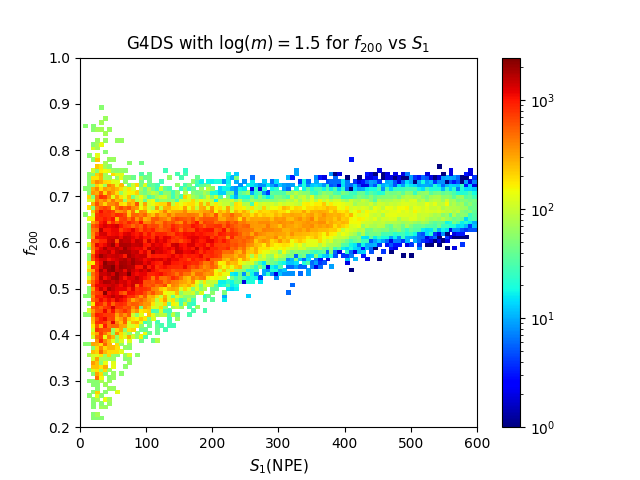
\includegraphics[scale=0.6]{./images/1.5/g4_f200_vs_s1.png}
      \caption{G4DS generated plot for $f_{200}$ vs $S_1$.}
  \end{subfigure}
  \begin{subfigure}{.5\textwidth}
      \centering\captionsetup{width=.9\linewidth}%
      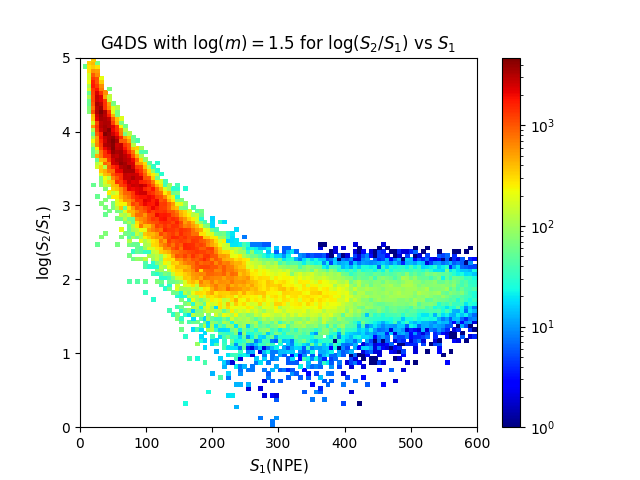
\includegraphics[scale=0.6]{./images/1.5/g4_s1_over_s2_vs_s1.png}
      \caption{G4DS generated plot for log($S_2$/$S_1$) vs $S_1$.}
  \end{subfigure}
\end{minipage}
\begin{minipage}{\textwidth}
  \begin{subfigure}{.5\textwidth}
      \centering\captionsetup{width=.9\linewidth}%
      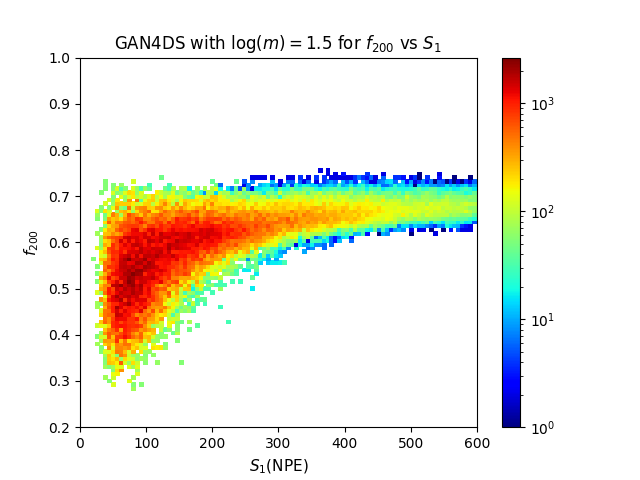
\includegraphics[scale=0.6]{./images/1.5/gan_f200_vs_s1.png}
      \caption{GAN4DS generated plot for $f_{200}$ vs $S_1$.}
  \end{subfigure}
  \begin{subfigure}{.5\textwidth}
      \centering\captionsetup{width=.9\linewidth}%
      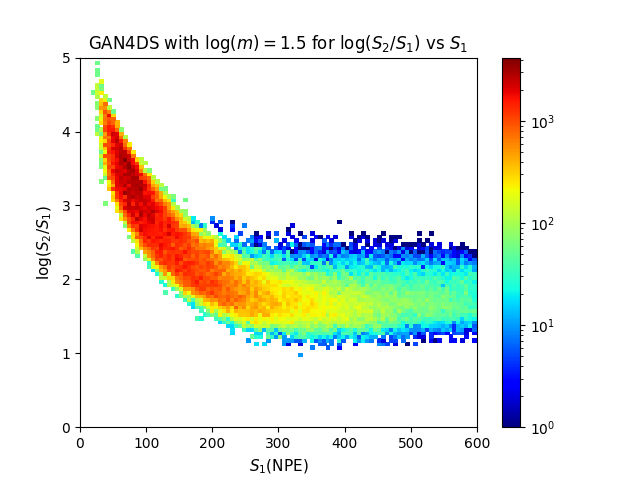
\includegraphics[scale=0.6]{./images/1.5/gan_s1_over_s2_vs_s1.png}
      \caption{GAN4DS generated plot for log($S_2$/$S_1$) vs $S_1$}
  \end{subfigure}
\end{minipage}
\begin{minipage}{\textwidth}
  \begin{subfigure}{.5\textwidth}
      \centering\captionsetup{width=.9\linewidth}%
      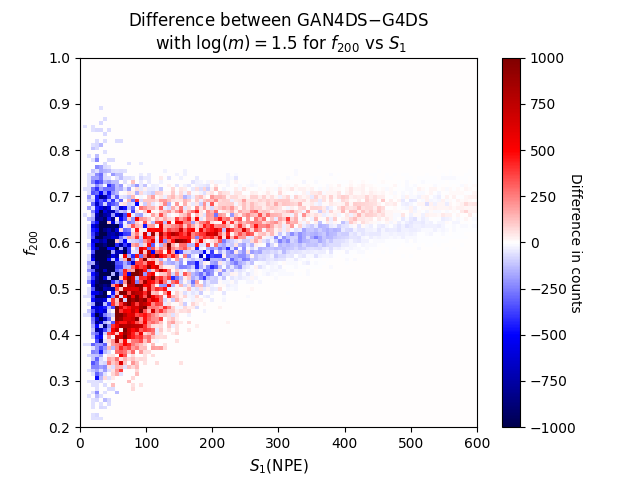
\includegraphics[scale=0.6]{./images/1.5/difference_f200_vs_s1.png}
      \caption{Difference per bin between GAN4DS $-$ G4DS generated data.}
  \end{subfigure}
  \begin{subfigure}{.5\textwidth}
      \centering\captionsetup{width=.9\linewidth}%
      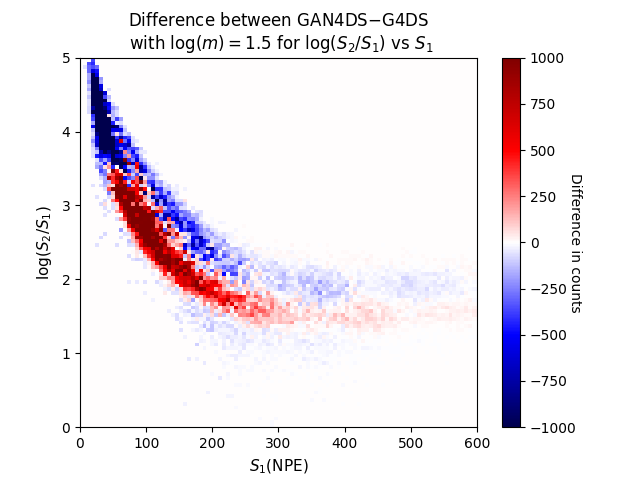
\includegraphics[scale=0.6]{./images/1.5/difference_s1_over_s2_vs_s1.png}
      \caption{Difference per bin between GAN4DS $-$ G4DS generated data.}
  \end{subfigure}
\end{minipage}
\caption{Results showing correlation learnt between the different variables by GAN4DS for log$(m)=1.5$.}
\label{fig:corr_results_1_5}
\end{figure}

\begin{figure}[H]
\centering
\begin{minipage}{\textwidth}
  \begin{subfigure}{.5\textwidth}
      \centering\captionsetup{width=.9\linewidth}%
      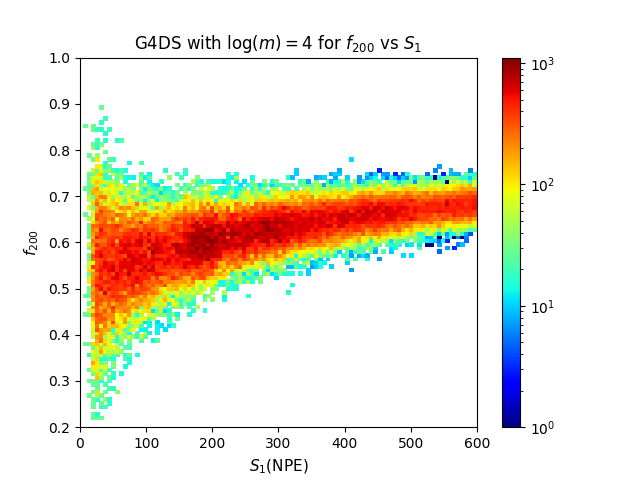
\includegraphics[scale=0.6]{./images/4/g4_f200_vs_s1.png}
      \caption{G4DS generated plot for $f_{200}$ vs $S_1$.}
  \end{subfigure}
  \begin{subfigure}{.5\textwidth}
      \centering\captionsetup{width=.9\linewidth}%
      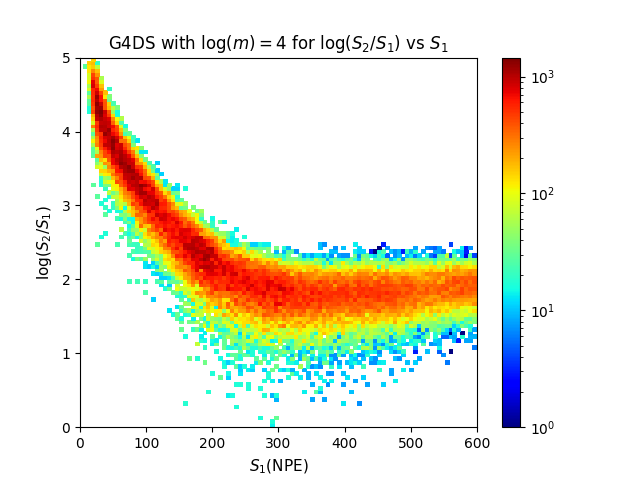
\includegraphics[scale=0.6]{./images/4/g4_s1_over_s2_vs_s1.png}
      \caption{G4DS generated plot for log($S_2$/$S_1$) vs $S_1$.}
  \end{subfigure}
\end{minipage}
\begin{minipage}{\textwidth}
  \begin{subfigure}{.5\textwidth}
      \centering\captionsetup{width=.9\linewidth}%
      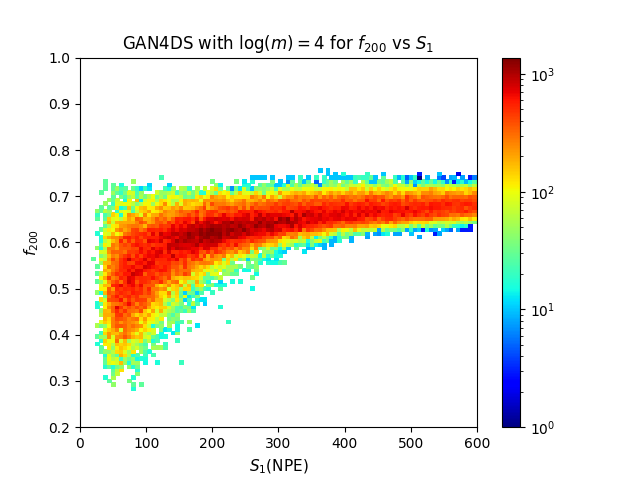
\includegraphics[scale=0.6]{./images/4/gan_f200_vs_s1.png}
      \caption{GAN4DS generated plot for $f_{200}$ vs $S_1$.}
  \end{subfigure}
  \begin{subfigure}{.5\textwidth}
      \centering\captionsetup{width=.9\linewidth}%
      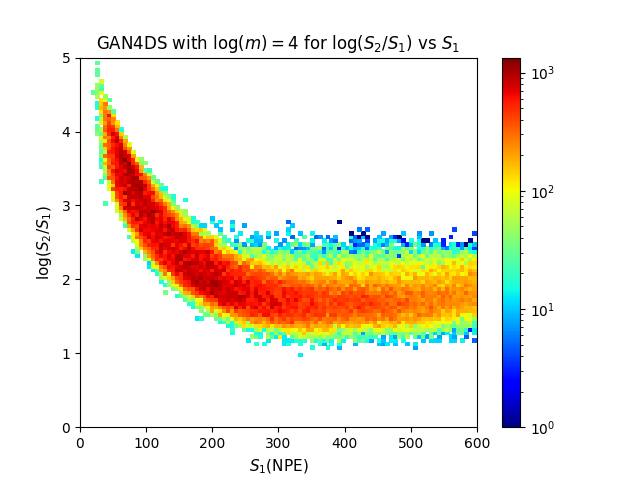
\includegraphics[scale=0.6]{./images/4/gan_s1_over_s2_vs_s1.png}
      \caption{GAN4DS generated plot for log($S_2$/$S_1$) vs $S_1$}
  \end{subfigure}
\end{minipage}
\begin{minipage}{\textwidth}
  \begin{subfigure}{.5\textwidth}
      \centering\captionsetup{width=.9\linewidth}%
      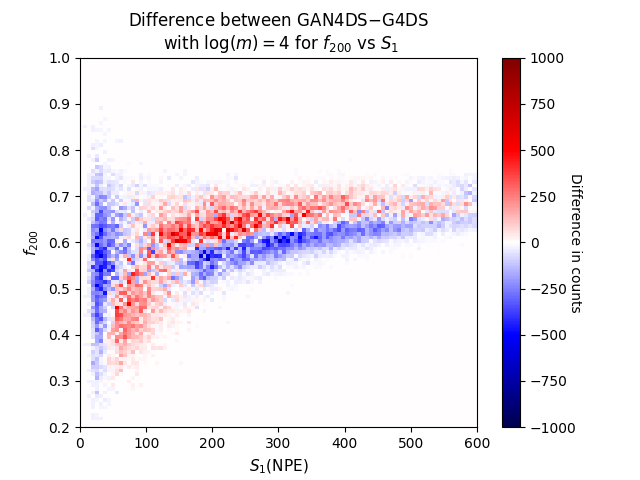
\includegraphics[scale=0.6]{./images/4/difference_f200_vs_s1.png}
      \caption{Difference per bin between GAN4DS $-$ G4DS generated data.}
  \end{subfigure}
  \begin{subfigure}{.5\textwidth}
      \centering\captionsetup{width=.9\linewidth}%
      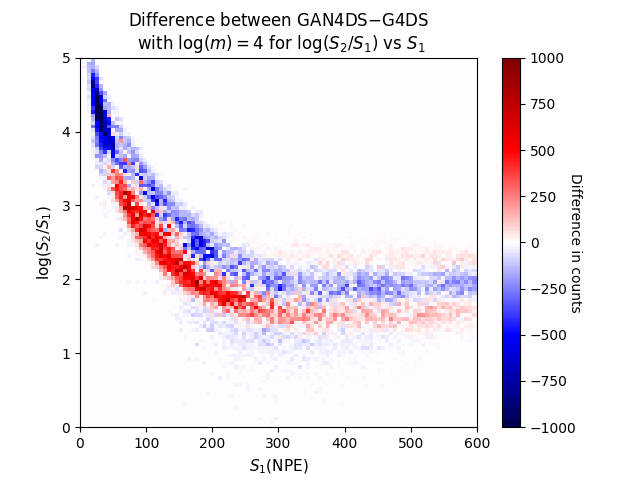
\includegraphics[scale=0.6]{./images/4/difference_s1_over_s2_vs_s1.png}
      \caption{Difference per bin between GAN4DS $-$ G4DS generated data.}
  \end{subfigure}
\end{minipage}
\caption{Results showing correlation learnt between the different variables by GAN4DS for log$(m)=4$.}
\label{fig:corr_results_4}
\end{figure}

\subsection{Accuracy Analysis}
\begin{figure}[H]
\centering
\begin{minipage}{\textwidth}
  \begin{subfigure}{.5\textwidth}
      \centering\captionsetup{width=.8\linewidth}%
      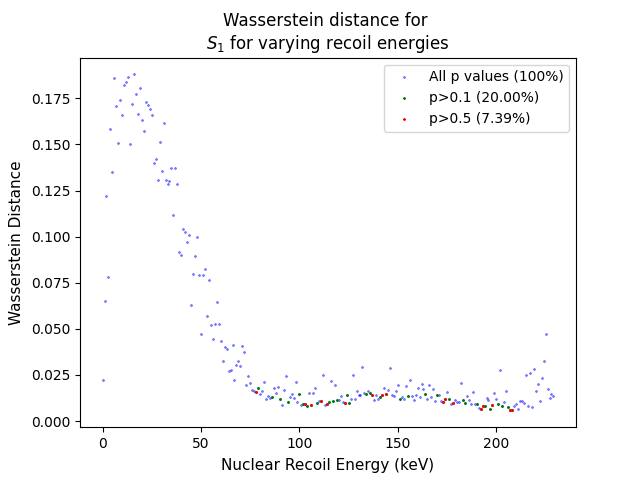
\includegraphics[scale=0.6]{./images/wasserstein_distance_s1.png}
      \caption{G4DS.}
  \end{subfigure}
  \begin{subfigure}{.5\textwidth}
      \centering\captionsetup{width=.8\linewidth}%
      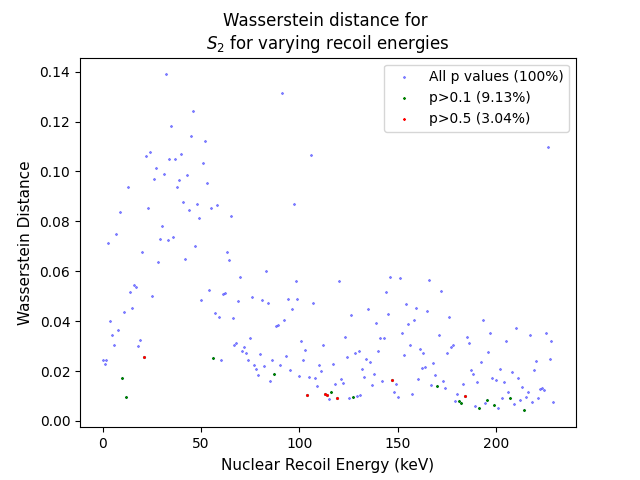
\includegraphics[scale=0.6]{./images/wasserstein_distance_s2.png}
      \caption{G4DS.}
  \end{subfigure}
\end{minipage}
\begin{minipage}{\textwidth}
  \centering
  \begin{subfigure}{.5\textwidth}
      \centering\captionsetup{width=.8\linewidth}%
      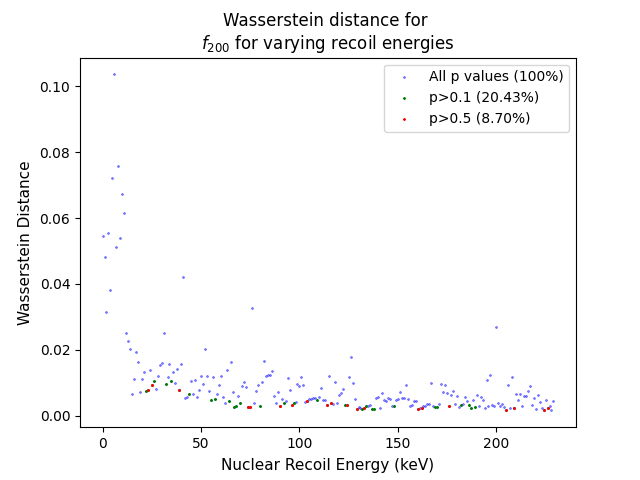
\includegraphics[scale=0.6]{./images/wasserstein_distance_f200like.png}
      \caption{G4DS.}
  \end{subfigure}
\end{minipage}
\caption{Wasserstein metric calculated on the GAN4DS and G4DS generated data for each variable for each energy. P values are
obtained by using a permutation test on geometric mean. In round brackets is the percentage of points that pass the significance threshold.}
\label{fig:wass_distance}
\end{figure}

Figure \ref{fig:wass_distance} shows the results of applying the Wasserstein metric \cite{ramdas2017wasserstein} on each variable for each nuclear recoil energy
between GAN4DS and G4DS.
The Wasserstein metric is often used to compare two distributions together and works on the amount of work/area needed to move around one distribution
to make it equal to the other.
The colours on the points of these plots signify another test we carried out.
Known as a permutation test \cite{pitman1937significance} \cite{efron1994introduction}, we calculate the geometric mean of the each two equal energy, equal variable distributions and take the absolute difference.
We then mix all the data points from the two and split them into two groups of random permutations of all the data points.
We then carry out again the absolute difference in geometric mean of the two groups and check if this is at least as extreme as the original geometric mean difference.
This is carried out for 1000 permutations and finally we end up with a probability that if we were to observe another value (have another generated distribution by GAN4DS)
this would have an absolute geometric mean difference with the real data at least as extreme.
This test is known as a two-tailed hypothesis test (since we do not know \textit{a priori} if GAN4DS will underestimate or overestimate G4DS data)
with the assumption of a Null hypothesis being true.
In our case the Null hypothesis is that the two distributions are the same.
Therefore, the value of p the permutation test returns is the confidence we have that we cannot reject the Null hypothesis.
We can never accept the Null hypothesis with this test but only reject it or fail to reject it.
\\
\par The first observation out of these plots is that the GAN reproduces training data much better at higher recoil energies
than lower ones.
This is seen both in the lower Wasserstein distance and the higher amount of points that pass
the permutation test's p significance value.
The even more interesting observation is that the relative distance between variables in the lower energy region
decreases from $S_1$ to $f_{200}$.
Recall, these variables were learnt successively and this behaviour seems to show a self-correcting learning behaviour
across variables, not only across epochs.
The pronounced spike in Wasserstein distance between G4DS and GAN4DS for lower recoil energies in $S_1$, seems to disperse for $S_2$ and
again becomes smaller in magnitude and shape, for $f_{200}$.
Essentially, if the GAN does not quite learn how to reproduce this Gaussian-like shaped data for $S_1$, the mistake
is not repeated as a whole for $S_2$, even though the neural network layout used for these two is the same.
Rather it appears the more variables trained on, the more we can actually see the GAN
getting better at reproducing these Gaussian-like shapes.
There is one caveat in that Wasserstein distances rely on areas so they might not be exactly comparable across different variables.
However, we do normalise each distribution before calculating each Wasserstein distance.
This is done by dividing both GAN4DS and G4DS variable distributions by the same normalisation value as described previously in Section 3.2.
Using this normalization makes the three plots in Figure \ref{fig:wass_distance} more comparable.
\\
\par Finally, these results suggest one could benefit in splitting the data around the 75 keV mark into two groups and actually
have a GAN for lower energies and one for higher ones since they are more comparable to each other.
This result also made us question what would happen if one were to insert $S_1$ again after $f_{200}$ has been learnt.
If the Gaussian-like distribution generation has been perfected with each variable, this would make $S_1$ even better than it was originally the first
time it was learnt.
This could potentially be extended to a completely different way of learning.
Instead of learning all the energies for one variable, one could shuffle the variables while keeping the number of energies the same and train over 10,000 epochs.
We suggest this could be one implementation, alternatively going through cycles of $S_1$, $S_2$ and $f_{200}$ until the distributions are
learnt for all three variables.
The only way to know whether these approaches or any other ones would work is to study them
so we hope this can be done in future iterations of this project.
\section{Final Remarks}
Last semester was focused on getting a proof-of-concept GAN working to learn $S_1$, $S_2$ and $f_{200}$ and we managed to show this could be done, alas, not efficiently.
What we have done this semester is make these algorithms scalable and stable and analysed both qualitatively and quantitively performance and accuracy.
We have tried multiple architectures and ultimately settled on the very new ARGANs.
Nevertheless, this is by no means
the only way to do it, nor the best, and we definitely encourage new architectures to be tried since this field of research is currently extremely active.
More work has to be carried out in the homogenous learning across all the nuclear recoil energy domain, especially for lower energies.
We suggest doing this by cycling through the variables being taught multiple times in a successive order since we hypothesise it could
really help the GAN converge over the whole energy domain.
\\
\par Future extensions to this project could include noise and background simulations and eventually all these combined in a signle GAN tih signal events.
An even larger extension would be to generate the individual photon responses by the sensors and PMTs which could then in turn produce the variables studied by us.
This could potentially be used at the same time to produce directionality predictions by making use of a classifier connected to the output of the GAN.
It would be a massive help to the current detector setup since, as of today, the detector does not produce such kind of information.
To conclude, we believe this project has produced tantalising results and hope our work will be continued by future iterations of the project.
\newpage
\printbibliography
\newpage
\section*{Appendix 1: Impact of Covid-19}
As requested by the University, I this is as brief statement about how the global pandemic has
affected our expected work and deadlines.
Speaking for myself, I have had to go back home in mid-March for fear the airports
back home in Malta and the UK would close.
As a matter of fact, a few days after, they did and I had to stay in mandatory quarantine in Malta for 14 days.
Due to the sudden nature of my departure I have had to leave many important documents, books and learning resources
in Manchester and, especially the first few weeks, this caused me great headaches to find backup resources.
Krishan and I used to meet up twice a week but ofcourse, with this situation ongoing, could not; so we instead resorted
to online platforms and I cannot say we have been impacted in this respect.
The same goes for access to project resources since all that could be done via SSH to the GPU cluster the
department of physics has.
Finally, we managed to reach all our planned milestones up until the week I had to leave, after which,
we have struggled to create new parts but rather focused on polishing all the work we had done.
This was not only due to the Covid19 outbreak but was definitely the largest factor when it came to
not being able to properly plan ahead and discuss everyday what the next steps were, like we used to do in the weeks before.

\end{document}
